\chapter{\label{ch:4-ams}The American monsoon system in UKESM1 and HadGEM3}


This chapter evaluates the representation of the AMS in the CMIP6 models: UKESM1 and HadGEM3. The pre-industrial control, historical and AMIP experiments are evaluated highlighting the role of large and regional-scale biases, horizontal resolution and Earth System processes for the representation of the monsoon dynamics and teleconnections.
This chapter is based on the publication: \cite{garciafranco2020} in which all the analysis was performed by the lead author. % except for the interpretation and 



 % Model assessment and validation is also important for this purpose as this process 

\section{Introduction}

The response of regional monsoons to greenhouse forcing remains an open question \citep{zhou2016,pascale2019} because the observational record is too short to exhibit significant trends but also because biases in GCMs increase uncertainty in future model projections.
Although the thermodynamical response to greenhouse forcing in the tropics seems to be relatively well constrained, the dynamical response is less clear \citep{shepherd2014}. The American Monsoon System (AMS) dynamics are shaped by regional features which means that in order to understand the  precipitation response to greenhouse forcing in a monsoon region, we need to better understand regional model biases and dynamical responses to a forcing. % for monsoons. 

The assessment of climate models in monsoon regions is key to understanding current and future changes to the water cycle in the tropics. However, and despite current recognition as a monsoon, model assessments of the AMS are scarcely done in each CMIP phase.  These studies only provide a general view of the biases of each generation of models \citep[see e.g.][]{geil2013,ryu2014}. However, a deeper evaluation of individual models can be used to provide better insight into the processes associated with climatological biases in the large-scale circulation and ultimately better understand the causes for the model biases in the AMS regional features. 

For example, in the South American Monsoon, CMIP5 models improved from the CMIP3 phase in their simulations of the distribution of precipitation during monsoon maturity and exhibited an improved seasonal cycle \citep{jones2013,yin2013}. However, some biases such as the underestimation of rainfall in the central Amazon have persisted from the first generation of GCMs up until CMIP5 \citep{li2006,yin2013}. \added{The geographic distribution of rainfall during  austral fall and several characteristics of the South Atlantic Convergence Zone (SACZ) and South American Low-Level Jet (SALLJ) are also poorly represented in CMIP5 in spite of their importance for the SAMS \citep{van2015dynamical,zilli2019,jones2019recent,zilli2021rossby}.} However, these studies provided little evidence as to the reasons for the improvements or the remaining biases in the models. 
A clear motivation to evaluate models in the South American Monsoon is that the accurate simulation of the geographic distribution and seasonality of rainfall in the Amazon rainforest is a relevant issue due to the impact of the rainforest on climate and society \citep[e.g.][]{li2006,malhi2009,yin2013}.
% and thus more research on the representation of the South American Monsoon is warranted.

Climate research in recent decades has aimed to reduce uncertainty in climate projections by improving GCMs, but different approaches taken by modelling centres are seemingly disconnected \citep{jakob2014}. One approach is to reduce horizontal grid spacing down to km-scale resolution to rely less on parameterizations and more on physical laws to represent clouds and convection \citep{palmer2019}. A second approach uses new explicit representations of Earth System processes to better characterise complex land-atmosphere-ocean biogeochemical cycles that may provide a better constraint on aspects of the climate such as climate sensitivity, a parameter that depends on the carbon cycle \citep{marotzke2017,sellar2019,andrews2019}. Finally, recent modelling centres have chosen to include  stochastic  parametrisations of sub-grid processes since this approach has improved seasonal forecasts and may therefore improve climate projections \citep{palmer2019st}. 

Model validation and assessment is important to analyse the effect of new parameterisations and to highlight missing processes but also evaluate which route provides the more substantial model improvement, stochastic parametrisations, increased resolution or Earth System processes.
The focus of this chapter is to evaluate the CMIP6 experiments from HadGEM3 GC3.1 (GC3) and UKESM1 in the AMS. In this thesis, the AMS is considered to be composed of the North and South American monsoon systems, while also including the Midsummer drought region of southern Mexico and Central America as part of the AMS \citep[as in e.g.][]{vera2006,pascale2019}.

The remainder of this chapter is organised as follows. The following section described the data and methods used in this chapter. Section  \ref{sq:clim} compares modelled and observed climatological temperature, sea-level pressure and low-level wind fields,  whereas section \ref{sq:itcz} analyses the Pacific and Atlantic ITCZs. Section \ref{sq:precip} analyses the spatial and temporal characteristics of rainfall and convection in the AMS while section \ref{sq:enso1} documents the simulated teleconnections of ENSO. A summary and discussion of the results is provided at the end of the chapter.

\section{Methods and data} 
\label{sq:meth_ch4}
The model assessment of this chapter will use a range of experiments from the MOHC, described in section \ref{sq:modeldata} using the HadGEM3 and the UKESM1 models. The experiments from HadGEM3 run at N96 (labelled GC3 N96) and N216 (labelled GC3 N216) resolutions are used to evaluate the role of horizontal resolution whereas Earth System Model UKESM1, which is run at N96 resolution in all the experiments, is used to evaluate the effect of representing atmospheric chemistry and other processes for the representation of the monsoon. 
In this chapter, the term low resolution will refer to both UKESM1 and GC3 N96 experiments whereas medium resolution refers to GC3 N216 experiments.% Note that in most figures depicting horizonal patterns only a handful of simulations is shown and in most cases this selection aims to exhibit the widest range of responses observed. 

The historical experiments are used to evaluate model skill in reproducing the observed period whereas the AMIP experiment from GC3 N96 is used to highlight the role of SST biases. The historical experiment data is used only in the 1979-2014 period to directly compare with the observed period.
All the observational datasets used in this chapter are described in more detail in chapter \ref{ch:3-methods} but in summary, the surface or near-surface air temperature data is taken from the CRU4 dataset, precipitation from TRMM, CHIRPS and GPCC and the rest of the diagnostics are from ERA5.

The climate indices of ENSO and the QBO used in this chapter were obtained by the following process. 
For ENSO, the deseasonalized and detrended time-series of the area-averaged SSTs (EN3.4 region [190-240$^\circ$W,5$^\circ$S-5$^\circ$N]) is used as an index to composite months into positive, negative and neutral phases. 
A month is determined to be in the positive phase (El Niño) when the index is higher than +0.65 K and a negative phase (La Niña) when the index is more negative than -0.65 K to select moderate to strong events. A neutral month is found where the magnitude of the index is smaller than 0.5 K and months with an index between 0.5 and 0.65 are discarded as they are borderline weak ENSO events or neutral cases.  Other indices, including the use of a 5-month running mean \citep{trenberth1998}, were tested without significantly changing the results.   Previous studies \citep[e.g.][]{menary2018,kuhlbrodt2018}  showed that the MOHC models reasonably simulate several characteristics of ENSO such as the period and SST patterns.

\added{ Principal component analysis (PCA) has shown that ENSO events may be separated into two categories: Central Pacific (CP) and East Pacific (EP) events \citep{cai2020}, which highlight where the peak SST anomaly is found in the Pacific Ocean. PCA analysis was used on deseasonalized SST fields in the equatorial [12$^\circ$S-12$^\circ$N] Pacific Ocean [120$^\circ$E-260$^\circ$E]. The E-index is computed from $(PC1-PC2)/\sqrt{2}$ and the C-index from $(PC1+PC2)/\sqrt(2)$.
EP (CP) events were defined where the E-index (C-index) was greater than 1.}

\added{The SACZ is evaluated in these models using the Empirical Orthogonal Function (EOF) methodology \citep{carvalho2004,jorgetti2014}. First, active days are constructed by  computing the first EOF of the monthly-mean deseasonalized OLR and, then, the daily OLR, previously filtered to remove periods higher than 99 days, is projected on the EOF pattern to produce a time series of pseudo-principal components. Active SACZ days are found when this time series of pseudo-PCs is greater than 1, and the persistence is measured as the number of continuous days where the time series is greater than 1.}



Similarly, for the QBO, the deseasonalized and detrended time series of the equatorially averaged [10$^\circ$S-10$^\circ$N] zonal-mean zonal wind at the 70 hPa level is used as the QBO index for both reanalysis and model data. The westerly phase of the QBO (QBOw) is determined when the index is greater than 2 m s$^{-1}$ and the easterly phase (QBOe) when the index is less than -2 m s$^{-1}$. 


%Therefore, this chapter compares the effect of increased horizontal resolution and Earth System processes  on the representation of the AMS in a climate model. In this chapter, in addition to the historical experiments which are more suitable for model assessment, both the pre-industrial control and atmosphere-only experiments are also used. 
%For example, HadGEM3 was run at two horizontal resolutions for CMIP6, and UKESM1 can also be directly compared to 

% 
%The validation of climate models is important for multiple purposes, for example, to evaluate the effect of new  % and the potential use of the models to answer outstanding questions of the monsoon long-term variability and teleconnections. 
%A principal use of climate models is their role in climate projections that aim to roughly predict the effect of a given forcing, i.e., greenhouse warming, over global and regional climate. 
%The robustness and confidence in model projections depends on the results from model assesment and validations.



%In this chapter, two resolutions of the climate model HadGEM3 are compared against UKESM1, which has the same dynamical core and physical parametrisations, but with additional components of the Earth System (see section \ref{sq:modeldata}). 




%Overall, very few studies have analysed the relative roles of large-scale biases for monsoon representation or the links between features such as the ITCZ or the Walker circulation and the AMS, which may be particularly important when understanding projected responses to forcing \citep{zhou2016,wang2017}. }

 
%C
% The next efforts to improve climate models include increased horizontal resolution, better parameterisations and/or the addition of processes in new models known as Earth System models \citep{eyring2016}.
 %The new phase of the CMIP project will include a range of new submissions which will include models with higher resolution and more Earth System models \citep{eyring2016}. A comparison and evaluation of simulations with increased horizontal resolution and Earth System models may suggest where modelling efforts are resulting in significant improvements in model representation of monsoons.

%
%\section{Climatological features}\label{sq:clim}


\section{Surface temperature and low-level wind} \label{sq:clim}

 \begin{figure}[t!]
\centering
 %\noindent
 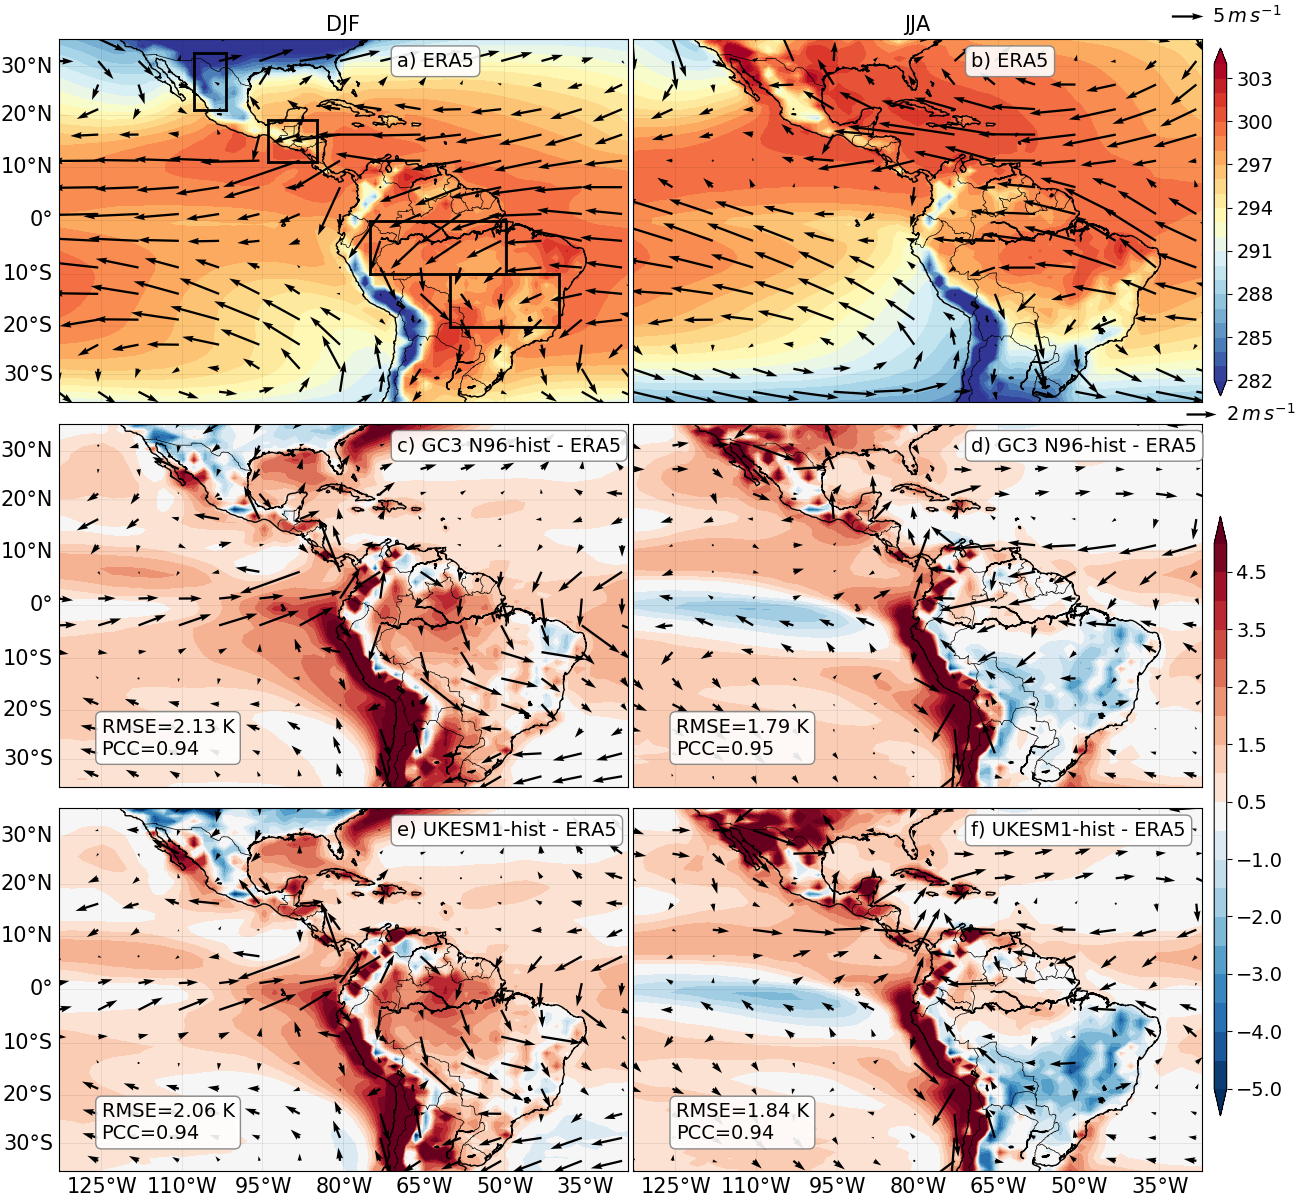
\includegraphics[width=\linewidth]{figures/fig1p2_f1a.png}
\caption[Temperature and SLP climatologies in UKESM1 and HadGEM3]{ (a, b) Temperature (color-contours in K) and wind speed (vectors) at 850 hPa DJF and JJA climatogies in ERA5. The biases are shown as the differences between the ensemble mean from the historical experiment of (c, d) GC3 N96 and  (e, f) UKESM1 and ERA5.
The climatogies and biases are shown for (a, c, e) boreal winter (DJF) and (b, d, f) boreal summer (JJA). Only differences statistically significant to the 95\% level are shown, according to a Welch t-test for each field. The key for the size of the wind vectors is shown in the top right corner of panels b) and d). The root-mean square error (RMSE) and pattern correlation coefficient (PCC) are shown on the bottom left of c-f.}
\label{fig:1}
\end{figure}


This section evaluates how these simulations represent the near-surface air temperature and low-level wind fields in the vicinity of the AMS region (Figures \ref{fig:1} and \ref{fig:1b}). % the climatology of DJF and JJA of ERA5 is shown in Figure \ref{fig:1}a, b.
The biases of the historical experiments, computed as the differences between the model and observed fields, are shown in Figures \ref{fig:1}c, d) for GC3 N96-hist and e, f) for UKESM1-hist.
 Only statistically significant differences are shown, according to a Welch t-test \citep{wilks2011}. The significance for simulations with multiple ensemble members is estimated first for each ensemble member and then combined into a single probability or p-value using Fisher's method \citep{fisher1992statistical}. Pattern correlations and root-mean square error (RMSE) are shown in Figures \ref{fig:1}c-f. % and in Table \ref{tab:s1}.
 


%\begin{table}[t!]
%\small
%\caption{\small Root-mean square error (RMSE) and pattern correlation coefficients (PCC) for each season and each model experiment. Near surface air temperature ($t2m$), wind components ($u$ and $v$) and mean-sea level pressure ($mslp$) are assessed against ERA-5 and precipitation ($pr$) against TRMM.}
%\begin{tabular}{p{1.05cm}|p{2.25cm}|p{1.10cm}p{1.10cm}p{1.10cm}p{1.10cm}p{1.10cm}p{0.9cm}p{1.05cm}p{1.05cm}} \label{tab:s1}
%  \textit{Variable}                  & \textit{Experiment}  & DJF RMSE & DJF PCC & MAM RMSE & MAM PCC & JJA RMSE & JJA PCC &  SON RMSE & SON PCC \\ \hline \hline
%t2m & GC3 N96 & 1.28 & 0.98 & 1.3 & 0.96 & 1.38 & 0.96 & 1.31 & 0.96 \\
%t2m & GC3 N216 & 1.05 & 0.99 & 1.07 & 0.98 & 1.02 & 0.98 & 0.98 & 0.98 \\
%t2m & GC3 Hist & 2.06 & 0.94 & 1.75 & 0.93 & 1.73 & 0.94 & 2.05 & 0.92 \\
%t2m & UKESM-hist & 2.03 & 0.94 & 1.77 & 0.93 & 1.8 & 0.94 & 2.0 & 0.93 \\
%t2m & GC3 AMIP & 1.17 & 0.98 & 1.12 & 0.97 & 1.2 & 0.97 & 1.2 & 0.97 \\
%u & GC3 N96 & 0.78 & 0.99 & 0.59 & 0.99 & 0.9 & 0.98 & 0.87 & 0.98 \\
%u & GC3 N216 & 0.78 & 0.99 & 0.59 & 0.99 & 0.9 & 0.98 & 0.87 & 0.98 \\
%u & GC3 Hist & 1.02 & 0.98 & 1.04 & 0.97 & 0.92 & 0.98 & 0.84 & 0.98 \\
%u & UKESM-hist & 1.04 & 0.98 & 1.01 & 0.97 & 0.91 & 0.98 & 0.82 & 0.98 \\
%u & GC3 AMIP & 0.96 & 0.98 & 0.77 & 0.99 & 1.18 & 0.97 & 1.09 & 0.96 \\
%v & GC3 N96 & 0.75 & 0.93 & 0.66 & 0.93 & 0.65 & 0.95 & 0.59 & 0.94 \\
%v & GC3 N216 & 0.6 & 0.96 & 0.5 & 0.95 & 0.57 & 0.96 & 0.54 & 0.94 \\
%v & GC3 Hist & 0.76 & 0.94 & 0.72 & 0.92 & 0.66 & 0.95 & 0.59 & 0.94 \\
%v & UKESM-hist & 0.75 & 0.93 & 0.69 & 0.92 & 0.65 & 0.95 & 0.6 & 0.93 \\
%v & GC3 AMIP & 0.67 & 0.95 & 0.52 & 0.95 & 0.68 & 0.94 & 0.61 & 0.93 \\
%mslp & GC3 N96 & 1.33 & 0.96 & 1.03 & 0.97 & 1.15 & 0.96 & 0.95 & 0.97 \\
%mslp & GC3 N216 & 1.11 & 0.97 & 0.9 & 0.97 & 1.1 & 0.96 & 0.89 & 0.97 \\
%mslp & GC3 Hist & 1.31 & 0.97 & 1.12 & 0.96 & 1.08 & 0.96 & 0.94 & 0.97 \\
%mslp & UKESM-hist & 1.4 & 0.97 & 1.15 & 0.96 & 1.14 & 0.95 & 0.99 & 0.97 \\
%mslp & GC3 AMIP & 1.15 & 0.97 & 0.87 & 0.97 & 1.09 & 0.96 & 0.93 & 0.97 \\
%pr & GC3 N96 & 2.02 & 0.79 & 2.24 & 0.71 & 1.62 & 0.9 & 1.69 & 0.86 \\
%pr & GC3 N216 & 1.58 & 0.88 & 1.72 & 0.85 & 1.4 & 0.93 & 1.57 & 0.89 \\
%pr & GC3 Hist & 2.05 & 0.78 & 2.49 & 0.64 & 1.69 & 0.88 & 1.69 & 0.86 \\
%pr & UKESM-hist & 1.96 & 0.8 & 2.39 & 0.66 & 1.71 & 0.88 & 1.62 & 0.87 \\
%pr & GC3 AMIP & 1.42 & 0.9 & 1.61 & 0.88 & 1.95 & 0.88 & 1.8 & 0.88 \\
%\end{tabular}
%\end{table}  

\begin{figure}[t!]
\centering
 %\noindent
 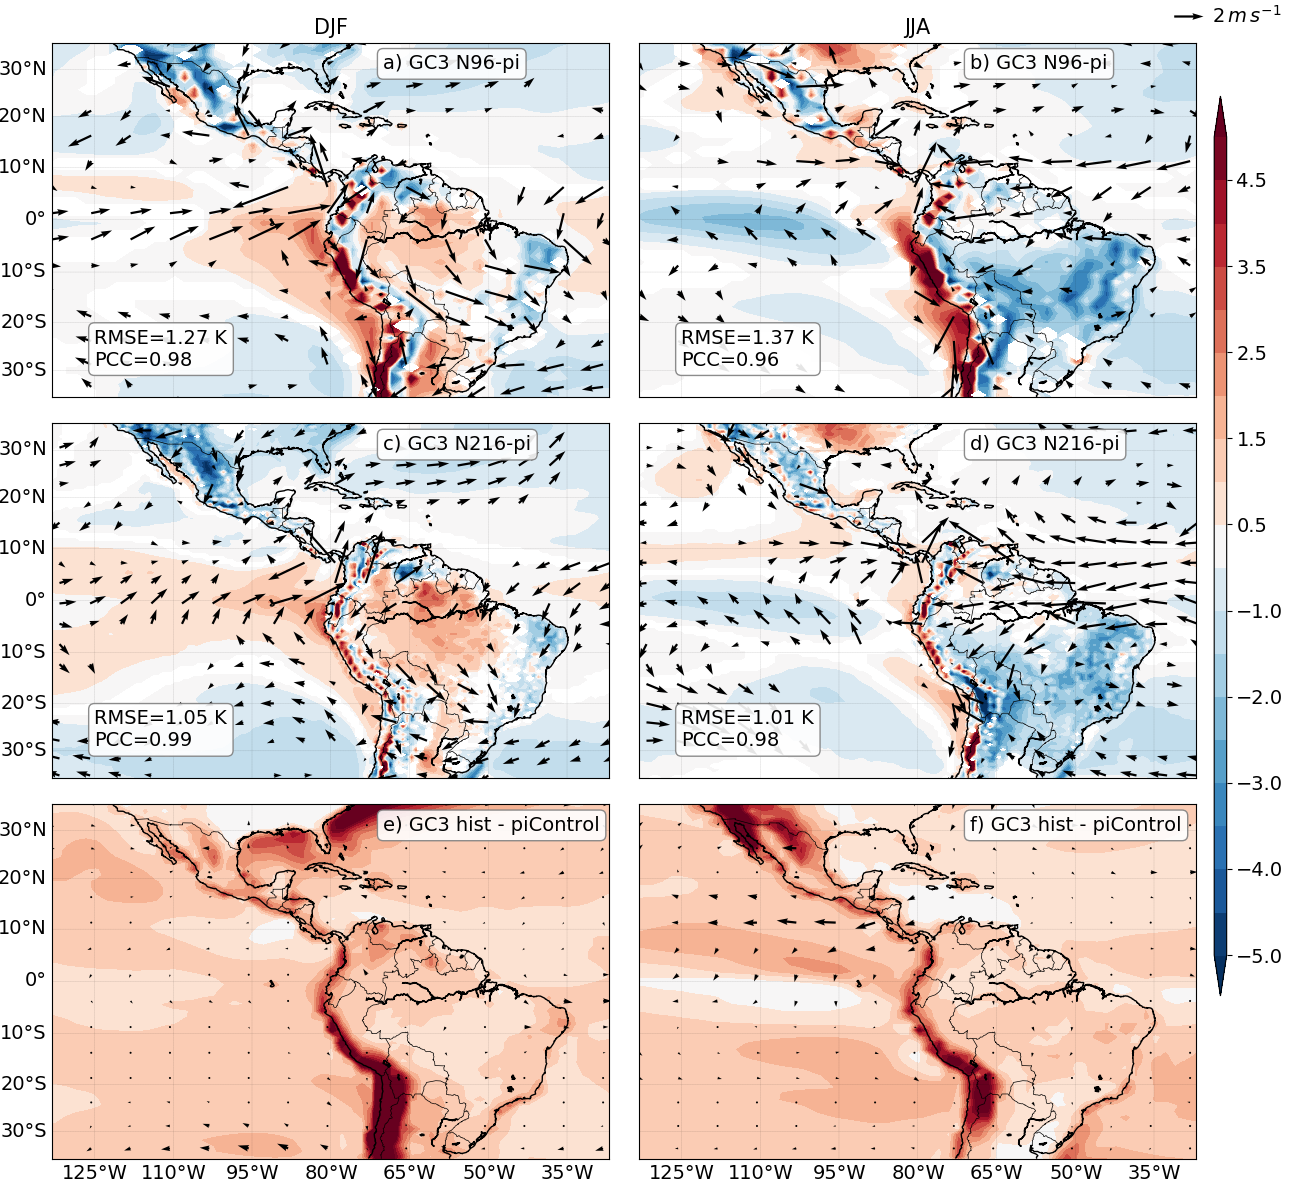
\includegraphics[width=\linewidth]{figures/fig1p2_f1b.png}
\caption[Temperature and SLP biases in UKESM1 and HadGEM3]{ As in Figure \ref{fig:1}, but showing the differences between the piControl simulations of (a, b) GC3 N96-pi and (c, d) GC3 N216-pi, and ERA5. (e, f) show the statistically significant differences between the historical (1979-2014) and piControl experiments of GC3.  The RMSE and PCC are shown on the bottom left of a-d.}
\label{fig:1b}
\end{figure}

 During DJF, the simulations show a colder-than-observed sub-tropical North America and a warm bias over the Amazon ($\approx +3.5$ K).
 The west coast of South America also shows a significant warm bias ($>+4$ K) in the historical simulations.
 The simulated circulation in austral summer in South America has a significant bias in the easterly flow coming from the equatorial and subtropical Atlantic.
 The low-level wind biases suggest a weaker easterly flow from the Atlantic into southeastern Brazil but also a strong southward flow from northern to southern South America.
  The South America Low-Level Jet, i.e., the low-level northwesterly flow in Bolivia, observed in Figure 1a, is stronger in the simulations.
   This stronger than observed jet is suggestive of a stronger moisture transport to the La Plata Basin, which has been associated with a drying of the Amazon and positive precipitation anomalies at the exit region of the jet \citep{marengo2012,jones2017}.
  % \citep


In turn, in boreal summer (Figures \ref{fig:1}d, f), positive temperature biases are observed in southwestern North America ($>+3.5 $ K), which are higher in UKESM1-hist than in GC3 N96-hist.
 The easterly flow west of Central America has a negative bias in UKESM1 suggesting a weaker flow that crosses from the Caribbean Sea into the East Pacific Ocean.
 %Both models show an anticyclonic anomaly in the region of the North Atlantic Subtropical High.
 Also in JJA, the simulated East Pacific surface temperatures are colder than observed for both historical experiments.      The inclusion of Earth System processes appears to make no  improvement on the low-level circulation biases. 

The temperature and low-level winds in the piControl simulations (Figures \ref{fig:1b}a-d) \added{are very similar} to the historical simulations.
 In DJF, the piControl experiments simulate a \added{warmer than observed Amazon whereas differences in the circulation in South America are essentially equal to the historical experiments. This result states the magnitude of the bias relative to the impact of forcing in these simulations. Note, instead, thate these differences with observations are smallest in GC3 N216-pi, which suggests a notable impact with horizontal resolution.
 In JJA, the piControl simulations do not show the warmer northwestern North America observed in the historical experiments, suggesting that this feature is linked to historical forcing. However, the weaker zonal wind over the easternmost Pacific is present in both piControl and historical simulations, again suggesting that this is a notable model deficiency.}
 
 Figures \ref{fig:1b}e, f show the difference between the historical and piControl experiment of GC3 N96, illustrating the response to historical forcing in GC3 N96.
 The temperature response in austral summer in South America is observed as 1.5 K whereas in JJA in North America temperatures were 4 K higher in the historical experiment than in the piControl.
 The only significant difference in low-level winds, as a response to historical forcing, are the easterlies in the East Pacific Ocean during JJA, which are stronger in the historical simulation.
  A very similar temperature and wind flow pattern response to historical forcing was observed for UKESM1 (not shown) although of slightly different magnitude. %hereas the rest of the low-level wind

%The SLP and wind biases show that during boreal winter, a lower-than-observed SLP in southern South America of -2 hPa, is associated with a northwesterly wind anomaly into southeastern Brazil. This anomalous circulation is weaker in GC3.1 n216 than in the other two simulations.

\begin{figure}[t!]
\centering
 %\noindent
 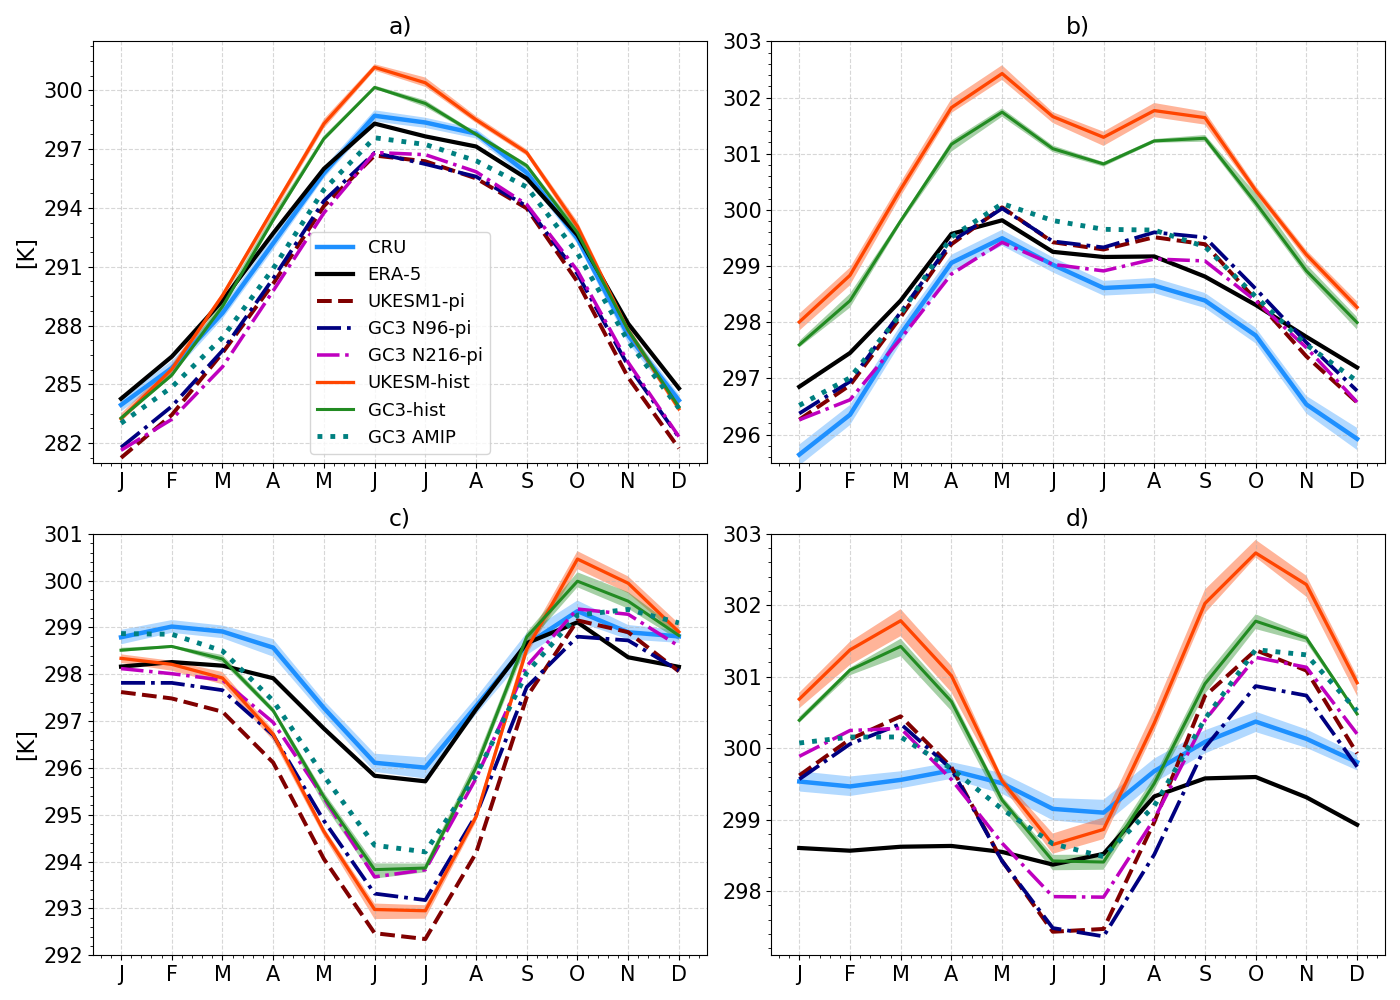
\includegraphics[width=\linewidth]{figures/p2fig2_v3.png}
\caption[Seasonal cycle of surface temperature in key monsoon regions]{ Monthly-mean temperature in the (a) North American Monsoon [19-35$^\circ$N,110-103$^\circ$W], (b) the Midsummer drought [11-19$^\circ$N,95-85$^\circ$W] (c) Eastern Brazil [20-10$^\circ$S,60-40$^\circ$W] and (d) the Amazon basin [-10-0$^\circ$S,75-50$^\circ$W] regions. The shadings for the CRU dataset represents the observational uncertainties and for the historical simulations the shading is the ensemble spread. The regions for this plot are shown in Figure \ref{fig:1}a. }
\label{fig:2}
\end{figure}

The seasonal cycle of temperature in key regions (depicted in Figure \ref{fig:1}a) of the AMS is shown in Figure \ref{fig:2}, comparing the simulations to ERA5 and the CRU4 dataset.
The temperature in the North American Monsoon region ranges from the boreal winter mean temperature of 12$^\circ$C to a maximum in June close to 27$^\circ$C.
Although the piControl simulated temperatures are colder than observed throughout the year, the models reasonably reproduce the seasonal cycle, which may be relevant for the simulated monsoon onset timing and strength \citep{turrent2009}. The historical experiments notably show a colder than observed winter and a warmer than observed summer compared to piControl experiments.

The piControl simulations show a colder-than-observed winter in southern Mexico and northern Central America. The historical experiments show a warming signal, when compared to the piControl simulations, of about 1.5 K in winter and 2 K in the summer in this region. Despite these biases, all the experiments follow closely the seasonal cycle in North and Central America.

However, the seasonal cycle in South American regions (Figures \ref{fig:2} c, d) of southeastern Brazil and the central Amazon shows notable temperature biases.
The simulations show a stronger than observed seasonal cycle, especially the historical experiments. For example, the modelled temperature difference between late austral winter and spring was $\approx$4 K whereas the observed temperature varies by less than 1 K in the same period. The models show a warm bias in the Amazon region (Fig. \ref{fig:2} d) which peaks in austral spring (SON), during the development of the monsoon \citep{marengo2012}.
In southeastern Brazil, the seasonal cycle is reasonably well reproduced but with a significant cold bias throughout the year which maximizes during austral winter (JJA), as models (e.g. UKESM1) simulate  a temperature 4 K lower than observed.
In all panels of Figure \ref{fig:2}, the historical experiments show a significant warming signal as a response to historical forcing, which is generally stronger in UKESM1 than in GC3 N96. 


The near-surface air temperature and the low-level wind structure during monsoon season are intertwined with the processes that lead to monsoon rainfall which means that the biases presented in this section will likely be related to biases in precipitation, e.g., through cloud feedbacks. For example, a biased wind structure in eastern Brazil as well as the positive warm bias in the central Amazon during DJF may indicate biases in the moisture transport and cloud cover that lead to the dry Amazon bias \citep{jones2013}. %The next section provides an assessment of a large-scale feature that is intimately related with monsoon rainfall:  the Intertropical Convergence Zones.

\section{The Atlantic and Pacific ITCZs and the SACZ}\label{sq:itcz}



The AMS is intertwined with the seasonal migration of the East Pacific and Atlantic ITCZ as the ITCZ largely determines regions of ascending and descending motions, moisture transport and is modulated by the hemispheric energy balance \citep{oueslati2013,li2014,zhou2016,cai2019pantropical}.The North American monsoon and MSD regions are influenced by the East Pacific ITCZ whereas the South American monsoon is affected by the Atlantic ITCZ \citep{yoon2010atlantic,marengo2012}. 
Three simulations are evaluated in this section: two low-resolution (N96) runs, the ensemble-mean UKESM1-historical, the ensemble mean GC3 AMIP and a medium-resolution run, GC3 N216-pi.
Other simulations are not shown as all the coupled low resolution (N96) simulations from UKESM1 and GC3 N96 showed very similar precipitation and ITCZ characteristics whereas the AMIP and medium-resolution experiments showed notable differences to the rest. 


\begin{figure}[t!]
\centering
 %\noindent
 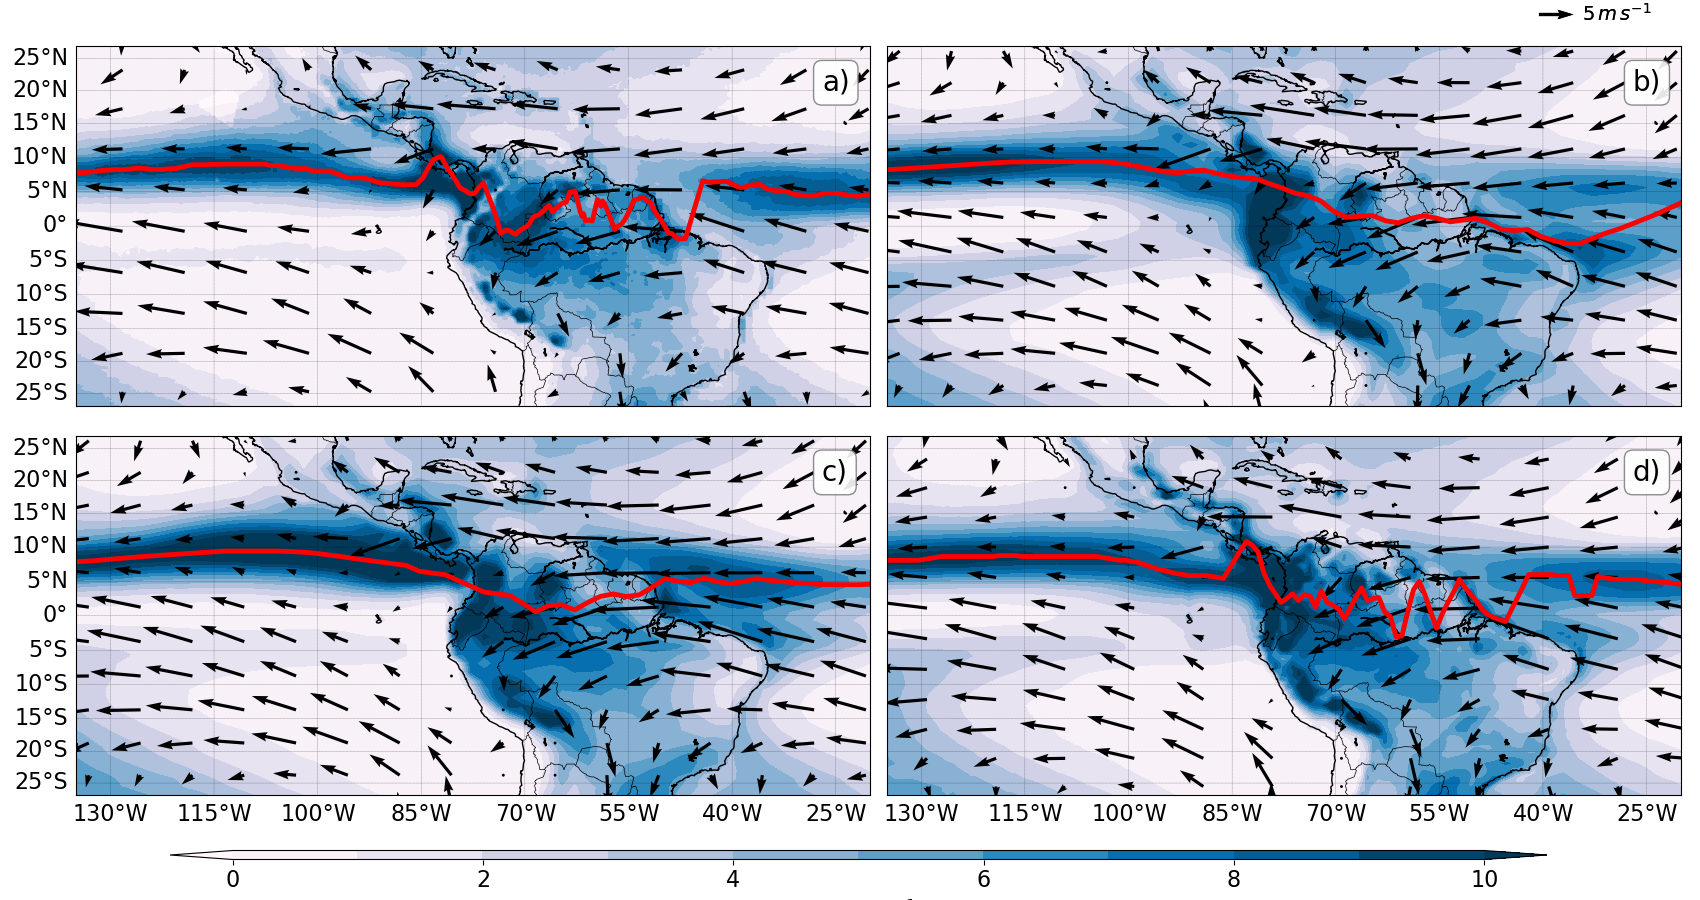
\includegraphics[width=\linewidth]{figures/itcz_clim_d.png}
\caption[Climatological precipitation and ITCZ position]{ Climatological precipitation [mm day$^{-1}$] and low-level wind speed (850-hPa) in (a) TRMM and ERA-5, (b) the ensemble-mean UKESM-historical, (c) GC3-amip and (d) GC3 N216-pi. The red line highlights the maximum rainfall for each longitude as a proxy for the position of the ITCZ.  }
\label{fig:3}
\end{figure}

The climatological ITCZ in TRMM (Figure \ref{fig:3}a) is found, on average, at 8$^\circ$N in the East Pacific and at 6$^\circ$N in the Atlantic.
All the simulations reasonably represent the climatological position of the East Pacific (EP) ITCZ; however, the modelled Atlantic ITCZ near the coast of Brazil is found south of the equator at 3$^\circ$S in the coupled model simulations.
The location of the ITCZ in GC3 N216-pi and the spatial distribution of rainfall is more consistent with TRMM dataset than the rest of experiments.
Rainfall near the Amazon river mouth is significantly larger in the low-resolution simulations than in the TRMM dataset. 
 However, the GC3 AMIP shows the best agreement with TRMM in ITCZ position and rainfall distribution. 

\begin{figure}[t!]
\centering
 %\noindent
 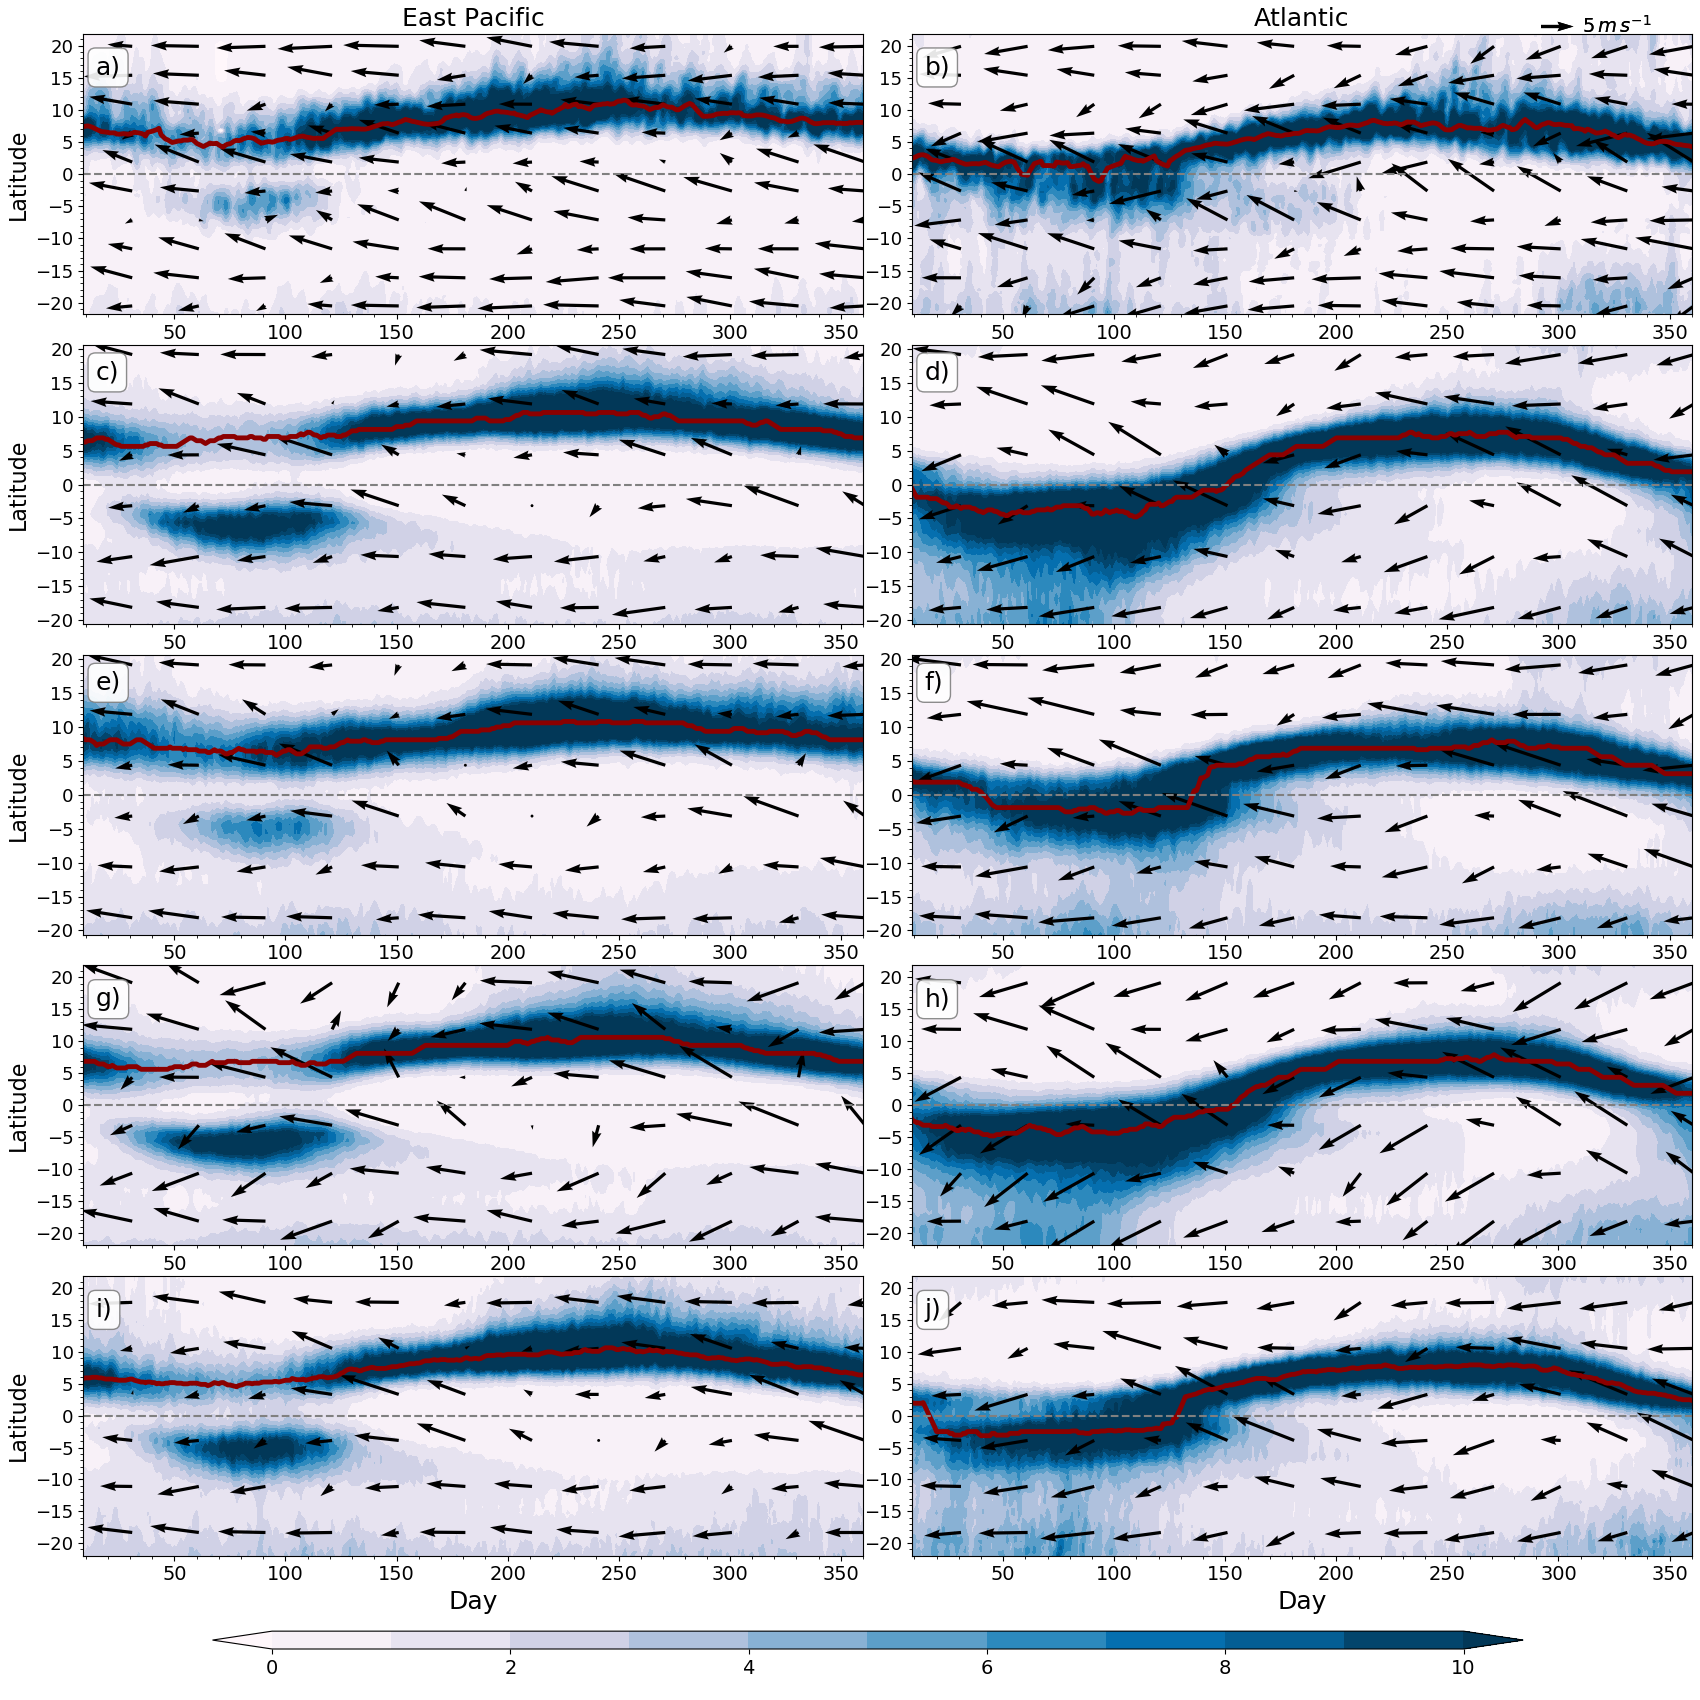
\includegraphics[width=\linewidth]{figures/fig3_p2_v3.png}
\caption[Seasonal evolution of Atlantic and Pacific ITCZ]{ Time-Latitude plot of daily mean rainfall (colour contours) and low-level wind speed (850 hPa) longitudinally averaged over the (a, c, e, g) East Pacific [150$^\circ$W-100$^\circ$W] and (b, d, f, h) Atlantic [40$^\circ$W-20$^\circ$W] Oceans. (a, b) show rainfall from TRMM and winds from ERA-5, (c, d) the ensemble-mean UKESM-historical, (e, f) GC3 AMIP, (g, h) GC3 N96-pi and (i, j) GC3 N216-pi. The red solid line shows the ITCZ as the latitude of maximum precipitation.  }
\label{fig:4}
\end{figure}


The seasonal cycle of the ITCZ location, precipitation rates and low-level winds in both basins are shown in Figure \ref{fig:4}, for TRMM, UKESM1-hist, GC3 AMIP, GC3 N96-pi and GC3 N216-pi.   %, two piControl and one historical simulations.
\added{The seasonal march of the ITCZ closely follows meridional migration of the solar insolation and the regional SSTs \citep{doi2012biases,donohoe2013}. An accurate representation of this migration requires a reasonable simulation of the coupling of the low-level circulation and SST gradients \citep{hastenrath2006,richter2014equatorial}.}

The EP ITCZ in observations (Fig. \ref{fig:4}a) migrates southwards during the first days of the year and is weakest and at its southernmost position at 5$^\circ$N around day 100 (mid-April).  
During boreal spring, the EP ITCZ migrates northward reaching a peak latitude and maximum rainfall at 10$^\circ$N by day 250, or early September. The EP ITCZ during boreal winter is weaker than during the rest of the seasons.
The low-level winds are predominantly easterly, which are stronger away from the ITCZ and weaker and convergent near the ITCZ position.
The position and seasonal migration of the EP ITCZ is reasonably well represented in the four simulations (Fig. \ref{fig:4}), but a noticeable bias in precipitation is observed in  boreal winter south of the equator in the coupled simulations. The modelled  low-level wind biases are characeterized as stronger winds converging toward the ITCZ during boreal summer and spring and diverging away from the equator during boreal winter. 

\begin{figure}[b!]
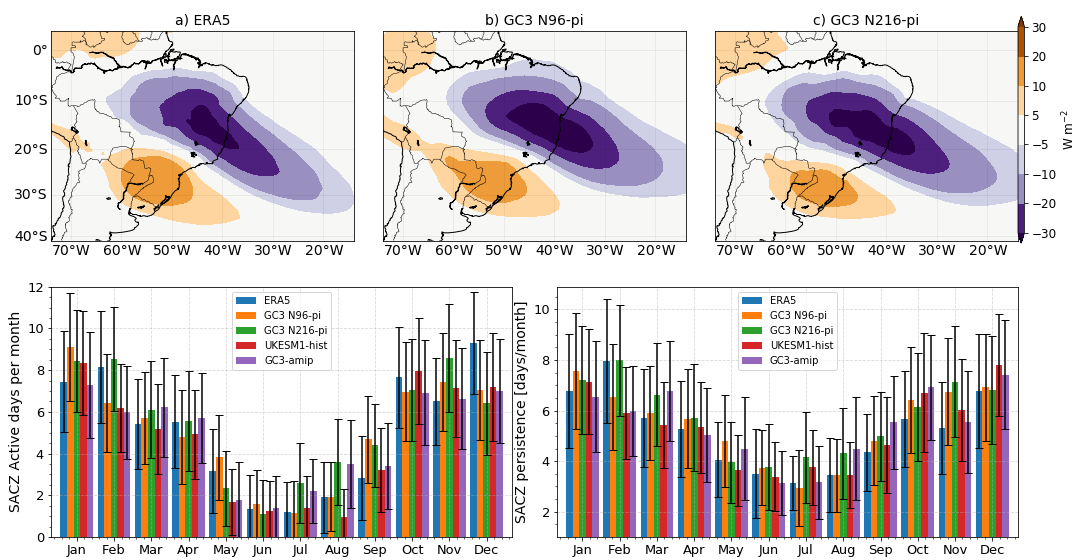
\includegraphics[width=\linewidth]{figures/saczanalysis.png}
\caption[SACZ assessment in UKESM1 and HadGEM3]{(a, b, c) OLR anomalies during active South Atlantic Convergence Zone (SACZ) events. (d, e) Frequency of active SACZ days and length of active SACZ events in reanalysis and model data, the standard deviation is shown as the error bar. }
\label{fig:sacz}
\end{figure}

The Atlantic ITCZ (Figure \ref{fig:4}b) has a similar seasonal cycle to the EP ITCZ, located at 4$^\circ$N at day 1 and migrates southwards at the start of the year reaching  its southernmost position at 0$^\circ$ at the end of March.
During boreal spring, the Atlantic ITCZ migrates north, reaching 8$^\circ$N at the start of boreal summer. In contrast to the EP ITCZ, the maximum rainfall in the Atlantic ITCZ does not weaken during any season. 
The position of the modelled ITCZ is generally biased south with respect to the observations.


The simulated ITCZ  crosses south of the equator during boreal winter, with maximum precipitation rates of 12 mm day$^{-1}$ found in the 0-10$^\circ$S region.
After boreal spring, the modelled ITCZ crosses back north of the equator and matches the observed ITCZ reasonably well for boreal summer and fall.
Low-level wind vectors near the Atlantic ITCZ (Figures \ref{fig:4}f and h) suggest a southerly bias north of the equator and a northerly bias south of 10$^\circ$S.
\added{Note that although there is a clear southward bias of the boreal winter ITCZ in this model, the GC3 N216-pi is top ranked amongst the CMIP6 cohort in the representation of the low-level trade winds and the SST gradients throughout the Atlantic \citep{richter2020overview}.}

%The biases in the Atlantic ITCZ can also be observed in the Walker circulation as significant negative $\omega$ and $q$ biases just north and south of equatorial South America indicative of weaker convective activity. The Atlantic Ocean in the simulations shows a biased negative $\omega$ (more ascent) south of the equator and a positive $\omega$ bias (less ascent) north of the equator in the low resolution simulations.
%The magnitude of the biases in the Atlantic ITCZ and overturning circulations described above were were associated with the horizontal resolution of the simulations. These biases were of similar magnitude in all the coupled model simulations run at the lower resolution N96, regardless of the type of experiment. However, these biases were reduced in the medium resolution experiments of GC3 N216 and in the GC3 N96 AMIP experiment which corrects SST biases (Figures \ref{fig:4}f, j). 

 The SACZ is a key element of the climate of the SAMS \citep{carvalho2004,jorgetti2014,van2015dynamical,zilli2019} that is not frequently assessed in climate models.  
 The mean representation of the SACZ features in these simulations, defined by the OLR empirical orthogonal function analysis (see section \ref{sq:meth_ch4}),  closely resembles the pattern found in ERA5 (Figure \ref{fig:sacz}). The SACZ active days and the persistence of the SACZ are also compared and found to be in relatively good agreement between reanalysis and model datasets.
 
The simulations from UKESM1, and GC3 N96 and N216 appear to reasonably simulate the spatial pattern of active SACZ days characterized by the low OLR in southeastern Brazil and higher OLR in the La Plata Basin. Similarly, the seasonal cycle of the frequency and persistence of SACZ active days is very well represented by the models with peak activity found from November through January and very little activity during austral winter. The impact that an accurate representation of the SACZ activity in GCMs has for representing short-scale variability of the South American Monsoon System is an open question, as the SACZ is rarely assessed in CMIP analyses.

GCMs have showed little improvement in their representation of ITCZs in CMIP phases\citep{oueslati2015} and this section shows that these biases are also found in these CMIP6 experiments. These biases are hard to improve because the position, strength and seasonal migration of the ITCZ are controlled by ocean-atmosphere feedbacks that intertwine the local and regional circulation with cloud-radiative feedbacks and the atmospheric and oceanic transport of energy \citep{schneider2014,oueslati2015,byrne2016,byrne2020}. \added{However, this evaluation of the model ITCZ representation could benefit from the the context that recent assessments of all CMIP6 models have provided which indicate that these MOHC simulations are top ranked in both the Atlantic and East Pacific \citep{tian2020,richter2020overview}.}

%This section shows that the CMIP6 MOHC models reasonably simulate the location of the East Pacific ITCZ but poorly represent the location of the austral summer Atlantic ITCZ and overestimate precipitation over the East Pacific ITCZ. The location and seasonal variability of the SACZ is also fairly well simulated by all the models. The implication of the results in this section for AMS precipitation will be addressed in the last section this chapter.


\section{Precipitation and convection in the AMS}\label{sq:precip}
%This section compares the spatial and temporal distribution of rainfall in four key regions of the AMS between observations and reanalysis, and the simulations, as well as other characteristics of convective activity, such as height and strength. %, are compared to better understand convective representation in this region.

\subsection{Mean seasonal precipitation}

\begin{figure}[b!]
\centering
 %\noindent
 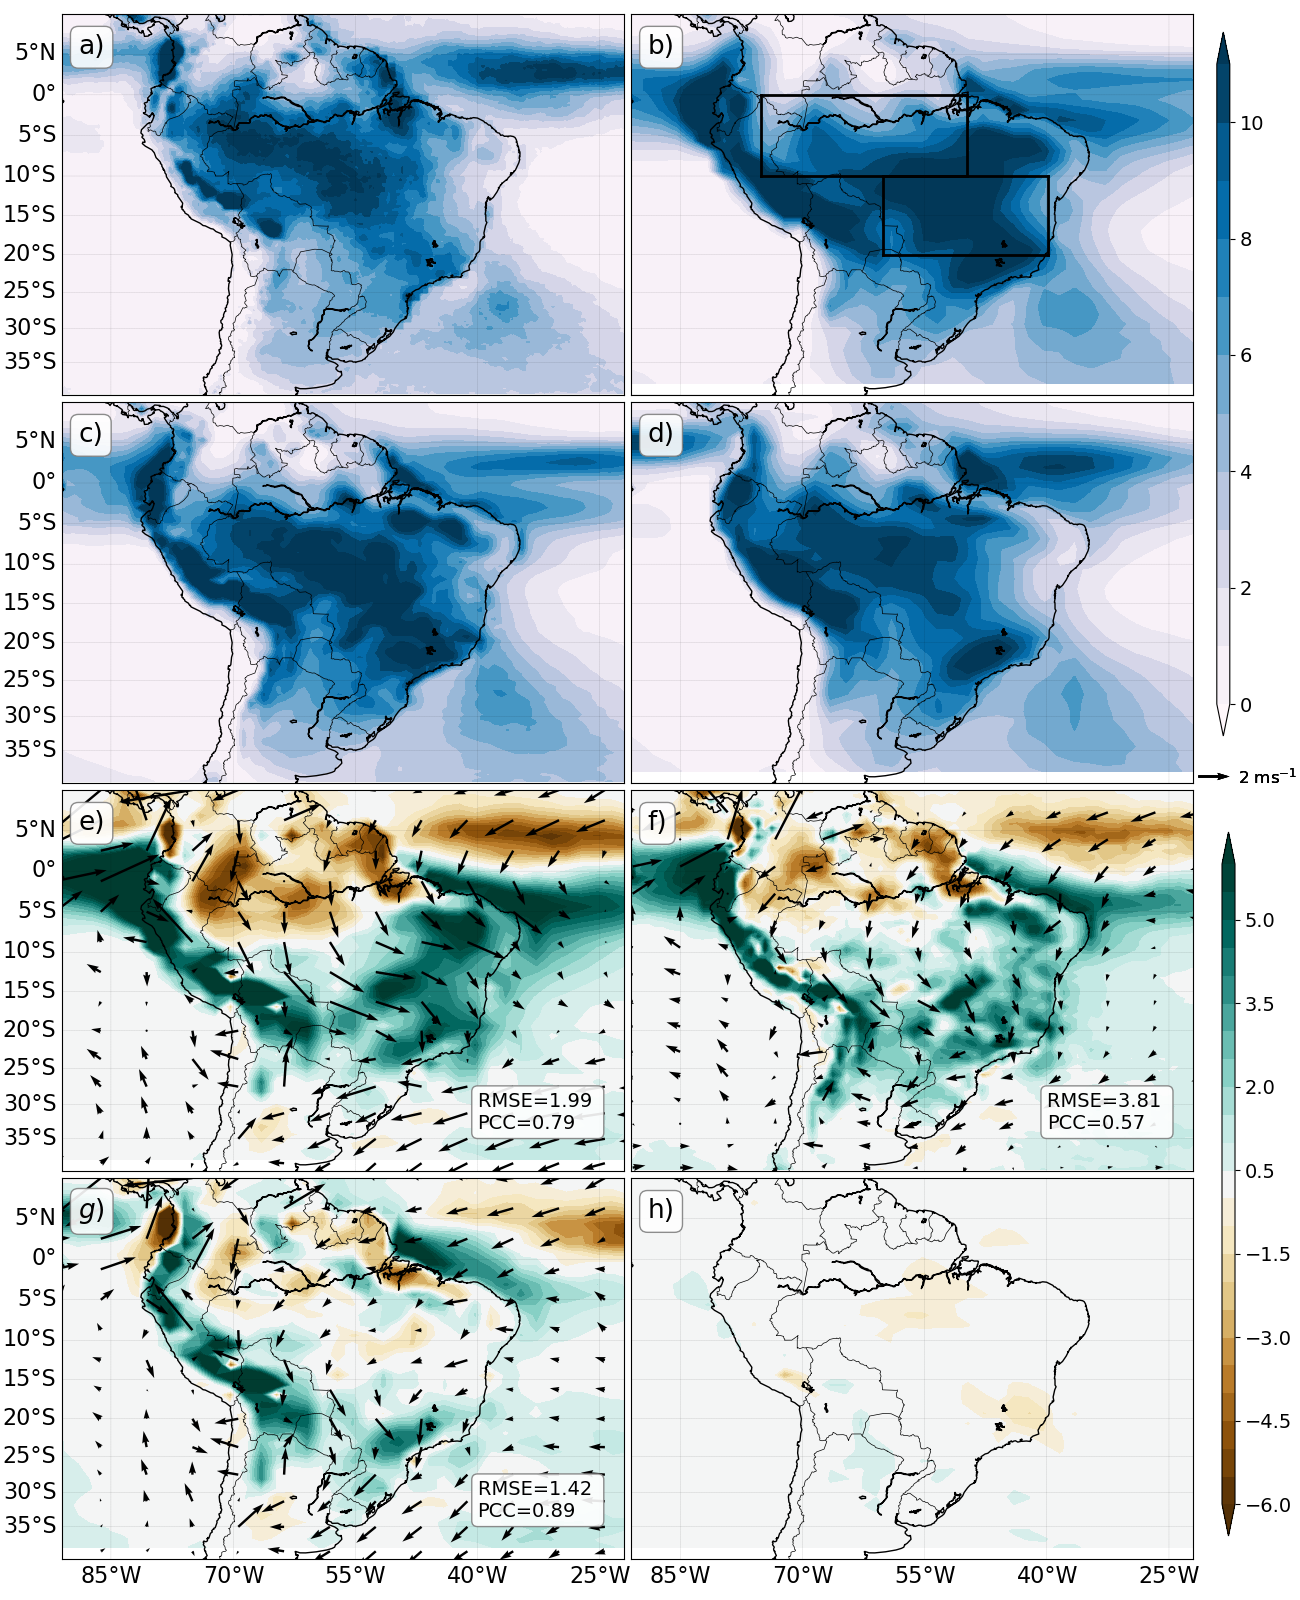
\includegraphics[width=0.875\linewidth]{figures/fig6.png}
\caption[Austral summer mean rainfall in the South American monsoon]{ DJF mean rainfall [mm day$^{-1}$] from (a) TRMM, (b) UKESM1-historical, (c) GC3 N216-pi and (d) GC3-amip. (e, f, g) show the statistically significant biases, i.e., differences between panels (b, c ,d) and (a) TRMM. (h) Precipitation difference between UKESM-historical and  UKESM1-pi, only statistically significant differences (95\% confidence level) are shown. In (e-g) in the 850-hPa wind biases are shown as vectors. }
\label{fig:6}
\end{figure}

  The austral summer (DJF) rainfall distribution in South America (Figure \ref{fig:6}) shows several noteworthy biases in the coupled simulations compared to TRMM. 
The maximum austral summer rainfall in TRMM
(Fig. \ref{fig:6}a) is found in a northwest-southeast oriented band from the core Amazon region into southeastern Brazil, the SACZ.
One main bias (Figs. \ref{fig:6}e-h)is the southward displacement of the Atlantic ITCZ, observed as positive (+5 mm day$^{-1}$) biases south of the equator and negative biases ($-$5 mm day$^{-1}$) north of the equator in the Atlantic. The models underestimate rainfall in the core Amazon basin by $-$3 mm day$^{-1}$ on average, and rainfall in southeastern Brazil is overestimated by more than +5 mm day$^{-1}$, approximately +100\% of the observed rainfall in this region.  
 
%The coupled simulations (e.g. Figure \ref{fig:6}b, c) overestimate rainfall in southeastern Brazil and underestimate rainfall in the core Amazon region.
 


 The precipitation biases are associated with a stronger northerly flow in South America, transporting moisture from the Amazon into southeastern Brazil and the La Plata Basin.   
The magnitude of these biases is smaller in GC3 N216 (Fig. \ref{fig:6}f) than in the low resolution simulations, such as UKESM1-hist.   The ensemble mean GC3 AMIP (Fig. \ref{fig:6}d) shows a better representation of the austral summer rainfall and circulation patterns, removing the main circulation biases (Fig. \ref{fig:6}g) of the coupled simulations.   
The response to historical forcing, illustrated by the difference between UKESM1-hist and UKESM1-pi (Fig. \ref{fig:6}h), is much weaker than the magnitude of the biases and is characterized by a weak drying of the Amazon and southeastern Brazil. Therefore, the magnitude of these biases are too large to have confidence in these drying responses to historical forcing. 


\begin{figure}[t!]
\centering
 %\noindent
 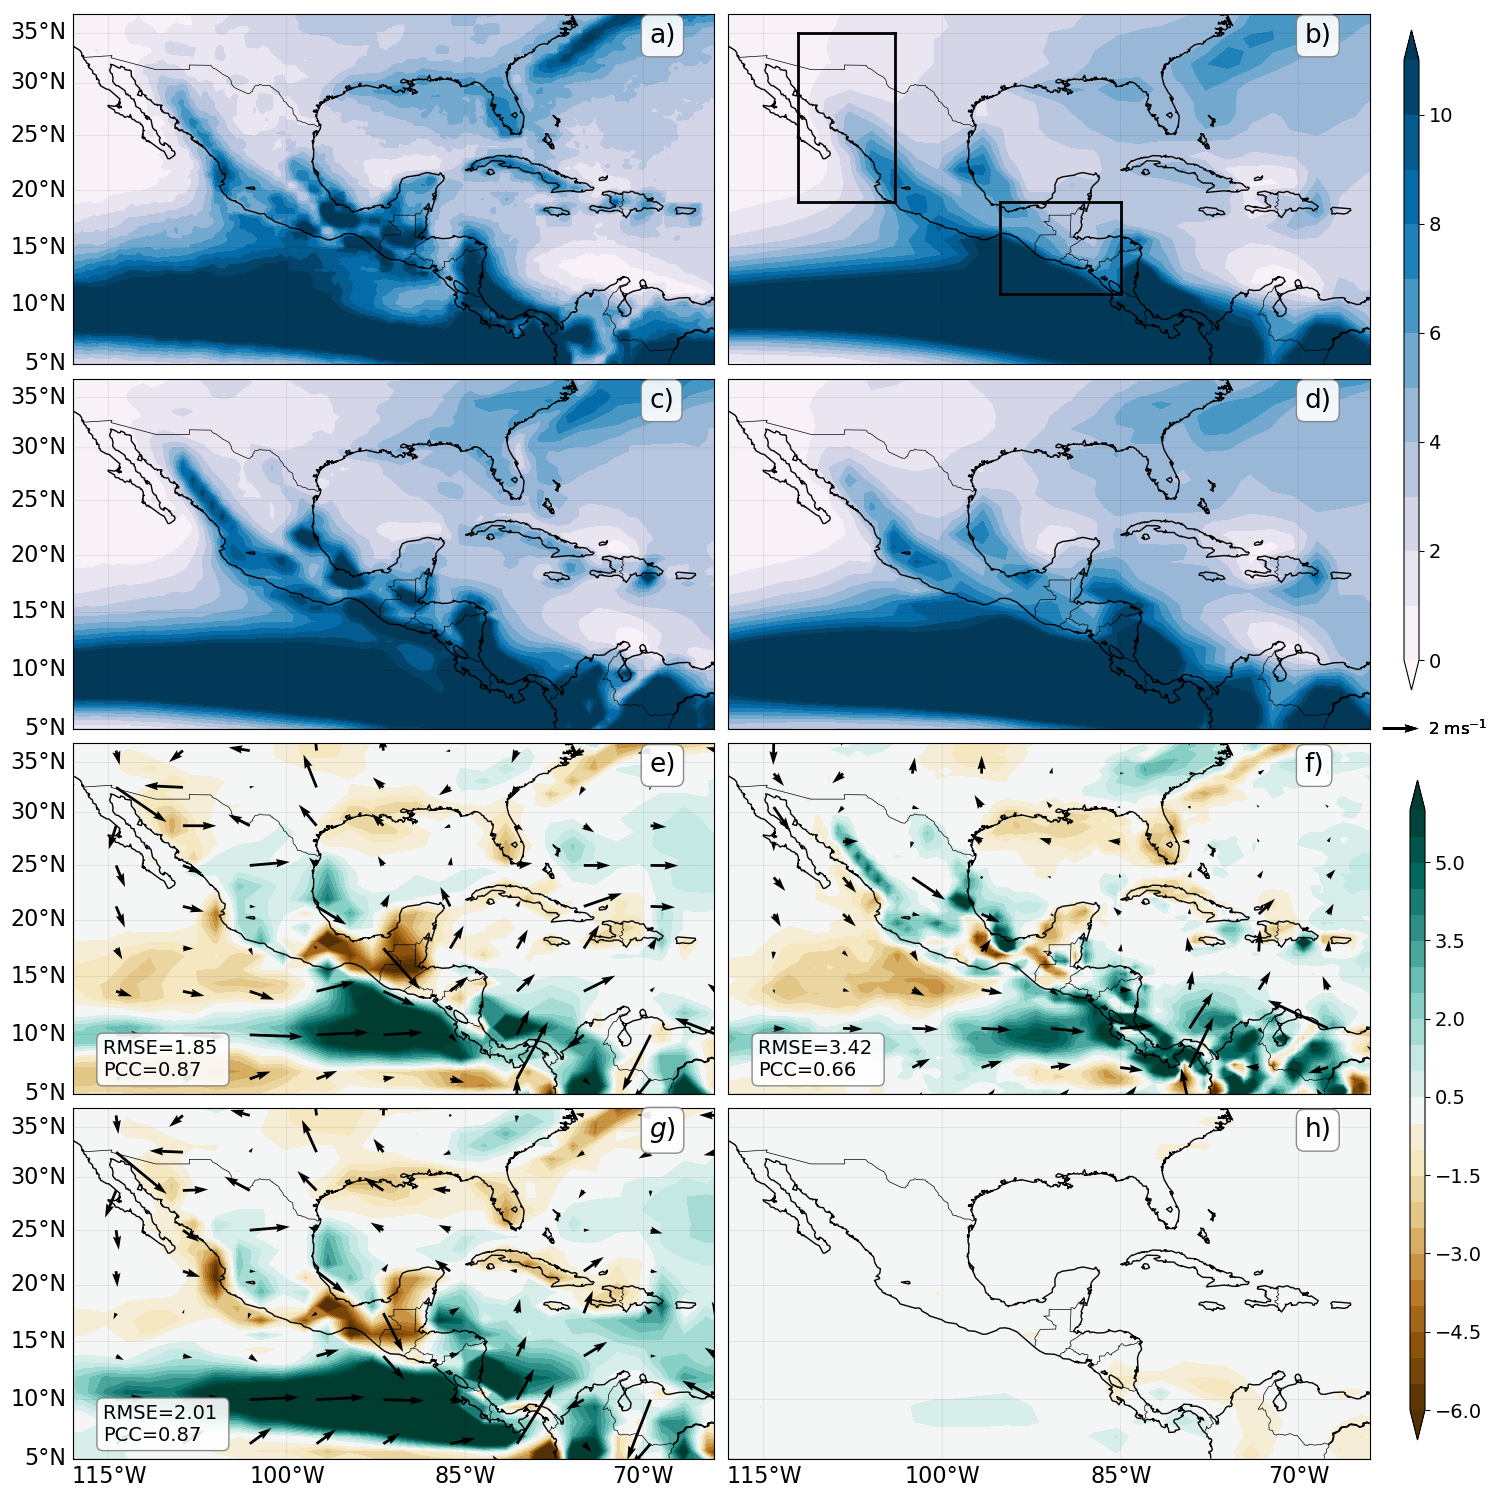
\includegraphics[width=0.9\linewidth]{figures/Fig8.png}
\caption[Boreal summer precipitation in the North American Monsoon]{ As in Figure \ref{fig:6} but for JJA in the northern part of subtropical America.   }
\label{fig:7}
\end{figure}

The modelled and observed JJA mean rainfall and biases for Mexico and Central America are shown in Figure \ref{fig:7}.
The main feature is the East Pacific (EP) ITCZ which extends north to 15$^\circ$N near the western coast of Mexico as a broad band of rainfall (>11 mm day$^{-1}$).
 The modelled EP ITCZ (Figures \ref{fig:7}e, f, g) rainfall is overestimated by more than 5 mm day$^{-1}$, especially in GC3-amip. This wet bias is associated with a westerly bias in the low-level circulation, suggesting a weaker flow from the Caribbean into the East Pacific.

The North American Monsoon can be observed as a band of precipitation across western Mexico. In the core monsoon region, near the Sierra Madre Occidental \citep{adams1997, zhou2016}, the JJA-mean rainfall is higher than 8 mm day$^{-1}$. %Several regions in southern Mexico also exhibit large seasonal mean rainfalls.
The distribution of rainfall in the North American Monsoon region is relatively well represented in all the simulations, as only a moderate wet bias (+2 mm day$^{-1}$) in western Mexico is observed.
The northernmost part of the North American Monsoon (southwestern US) is best simulated by GC3 N216-pi, as the other simulations show a dry bias in this region.
%This positive bias extends to southern Central America.
The low-resolution simulations (Figure \ref{fig:7}e) underestimate rainfall (-5 mm day$^{-1}$) over land in southern Mexico, Guatemala and Belize.
Rainfall in the Caribbean islands and Florida is underestimated (-1 mm day$^{-1}$) in all simulations.

In most cases for JJA in this region, the precipitation and wind biases were reduced in the medium-resolution simulation (Figure \ref{fig:7}f) and little-to-no difference was observed between UKESM1-hist and GC3 N96-hist (not shown).
The precipitation response to historical forcing is much lower than the biases (Figure \ref{fig:7}h) with no significant precipitation differences over land due to the historical forcing. % shows a decrease in precipitation.
 

\subsection{The annual cycle of rainfall}\label{sq:raincycle}

\begin{figure}[b!]
\centering
 %\noindent
 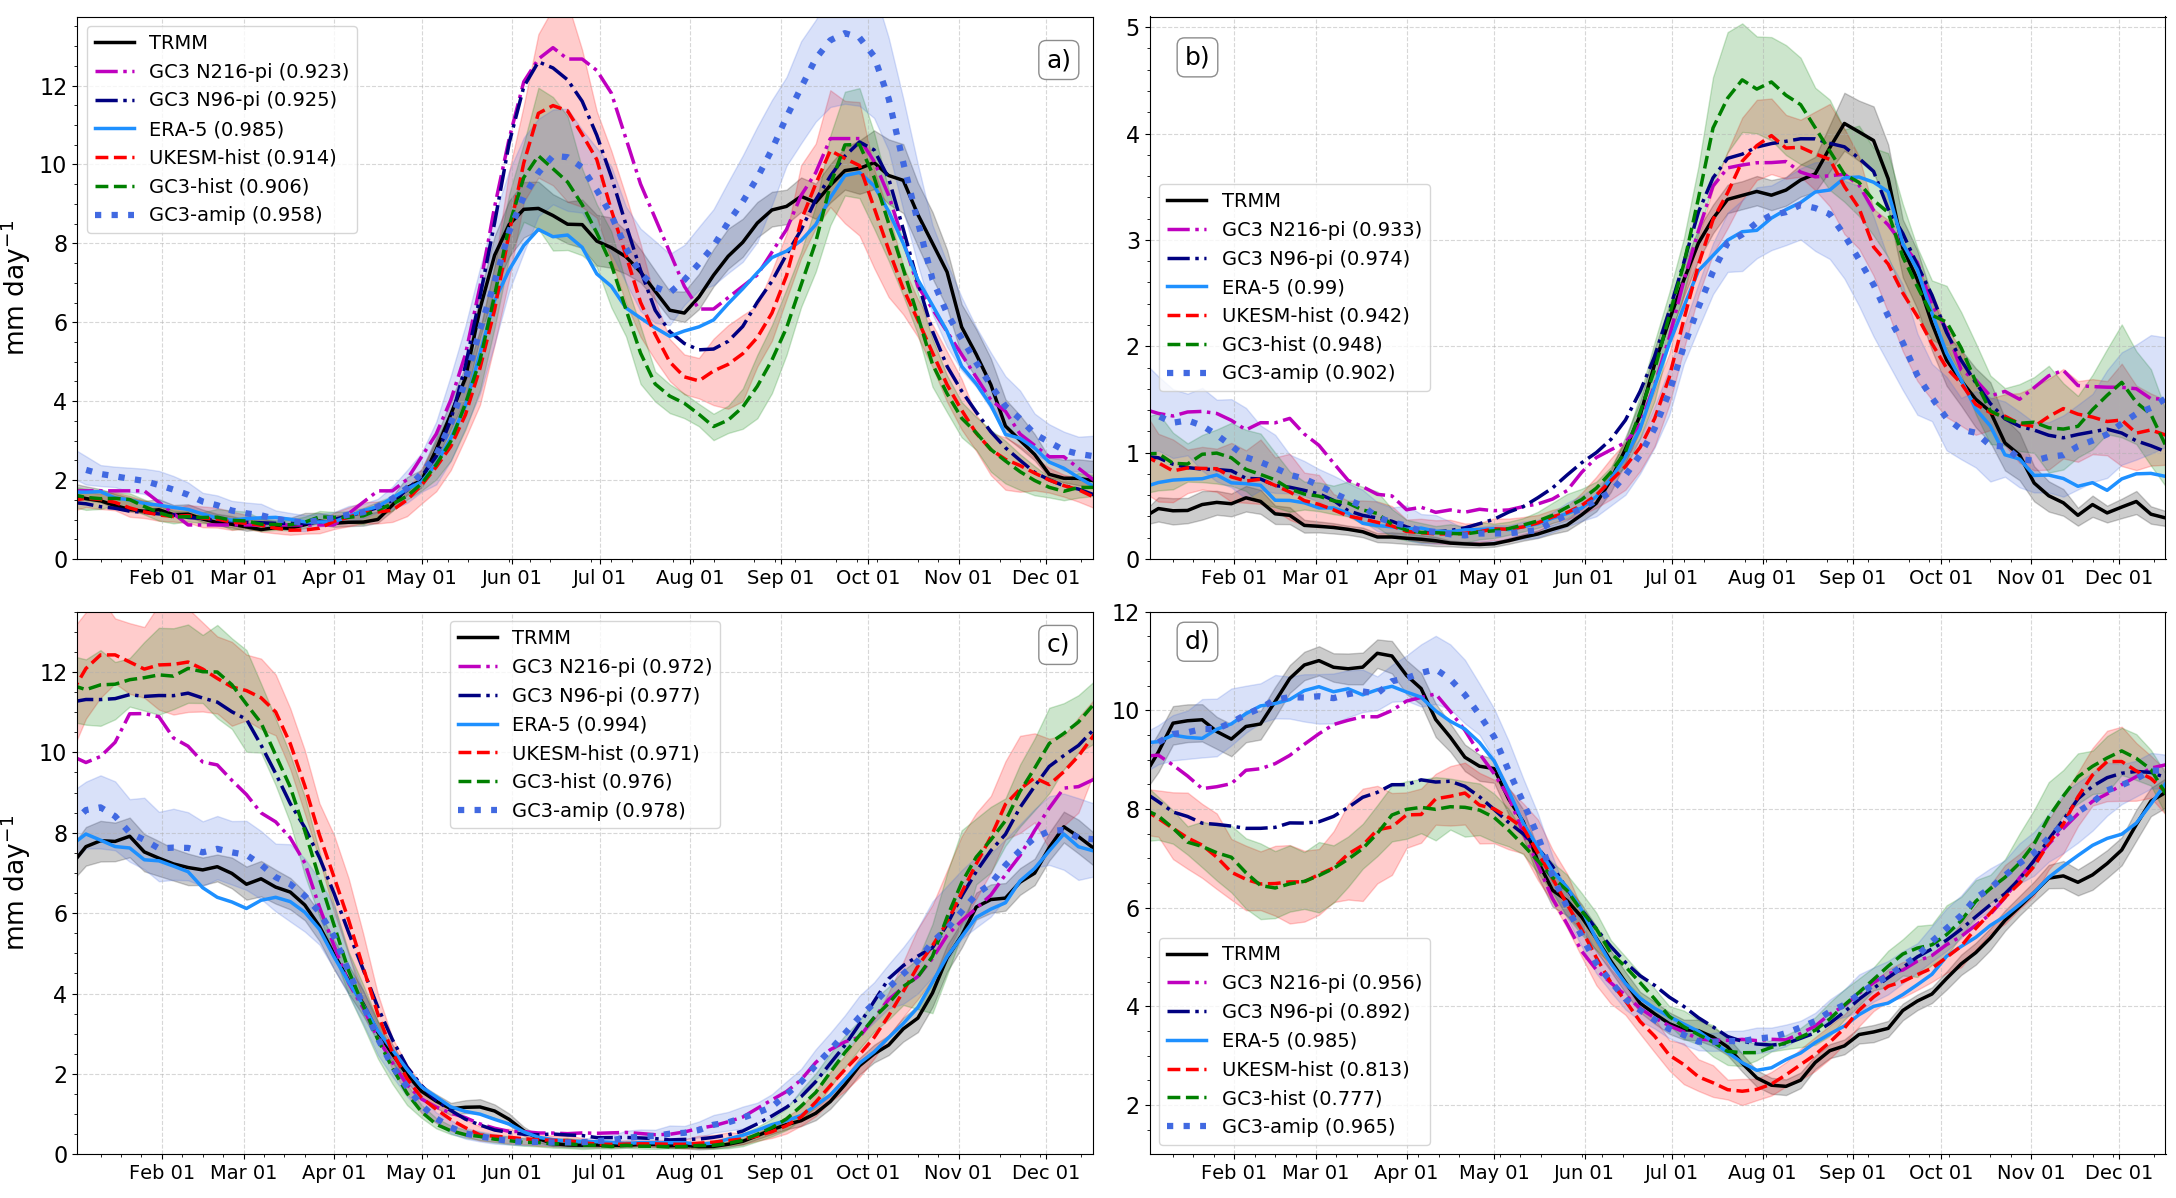
\includegraphics[width=1.0\linewidth]{figures/amipseasonalcycle.png}
\caption[Annual cycle of precipitation in different regions of the AMS]{Annual cycle of pentad-mean rainfall in the regions (a) the Midsummer drought, (b) the North American Monsoon, (c) Eastern Brazil and (d) the Amazon Basin. The regions are defined as in Figure \ref{fig:2} and are illustrated in Figure \ref{fig:7}b and Figure \ref{fig:8}b. The shaded regions represent observational uncertainty for TRMM and ensemble spread for the historical experiments. The correlation coefficient for each of the simulated seasonal cycles with TRMM is given in brackets in each panel.  }
\label{fig:8}
\end{figure}

%CMIP assessments typically evaluate rainfall model performance by inspecting area-averaged monthly-mean evolution of rainfall.
%However, this temporal resolution is not enough to properly evaluate the performance of a simulation, particularly in monsoonal regions where the dates of monsoon onset and demise have relevance for sectors such as agriculture.

Figure \ref{fig:8} shows the seasonal cycle of rainfall at the pentad (5-day) scale over the North American Monsoon, the  Midsummer drought (MSD), the Amazon and eastern Brazil regions. The correlation between TRMM and the model and reanalysis data (ERA5) is also shown in each panel. 

The seasonal cycle of precipitation in the MSD region in the simulations is well represented as all the simulations show the characteristic bimodal distribution, a feature that is difficult to simulate  for a climate model \citep{ryu2014}.
%This peculiar bimodal distribution of rainfall is characterised by a first rainfall maxima in June and a second maximum in late September, separated by a relatively drier period with a minimum at the start of August. The Midsummer drought bimodal distribution was only found in a handful of CMIP5 models \citep{yin2013}.
However, the magnitude of the first peak and second peaks of precipitation in the simulations are different. 
Most of the simulations show a wetter first peak than TRMM by 4 mm day$^{-1}$, and the AMIP simulation overestimates the second maximum of rainfall by 2-3 mm day$^{-1}$. Similarly, the differences between the first peak and the MSD and between the MSD and the second peak are more pronounced in the simulations. The timing of the MSD period is different in the models, as the simulations show the driest period taking place 10 days after TRMM and ERA5. %  All the simulations show different magnitudes of the first and second peak and the MSD precipitation, 
  

In the North American Monsoon (Figure \ref{fig:8}b), the observed seasonal cycle is characterized by a very long dry period from the November to June, which is followed by a sharp increase of rainfall around mid-June. The timing and strength of the onset of rainfall is well represented by all these simulations.
Moreover, the modelled and observed mean precipitation rates during monsoon maturity are $~$4 mm day$^{-1}$, from mid-July until early September, which suggests  the models can also reproduce the observed peak monsoon rainfall.
%The timing of monsoon retreat is also well represented by the simulations, as both modelled and observed rainfall decay during September.
   The historical simulations show a shorter wet season characterised by an earlier retreat of the monsoon rainfall and a positive bias (+1 mm day$^{-1}$) is found during late local fall and early winter, a feature present in most CMIP5 models \citep{geil2013}. % and that will be further explored in the following chapter. %For instance, GC3 N96-hist retreats on average around August 16th. 
%However, winter-time rainfall, before monsoon onset and after monsoon retreat, is overestimated by all the simulations, particularly the higher resolution GC3.1 N216 which has a positive bias of $~$2 mm day$^{-1}$ in early winter. 


The seasonal cycle of precipitation in eastern Brazil is characterised by a very wet summer ($\sim$8 mm day$^{-1}$) compared to a very dry ($\sim$0.2 mm day$^{-1}$) winter (Figure \ref{fig:8}c).
%The South Atlantic Convergence Zone has a centre of action over this region and thus controls several aspects of precipitation \citep{carvalho2004,marengo2012}.
%Rainfall in TRMM and ERA5 increases steadily from austral spring (September) to a maximum found in early January ($\sim$8 mm day$^{-1}$).
%Rainfall in this region decreases to $\sim$6 mm day$^{-1}$ by late March as the monsoon migrates northward and then sharply decreases in austral fall.
The models (Figure \ref{fig:8}c) show a positive bias during monsoon maturity. This bias was found to be of +4 mm day$^{-1}$ and +2.5 mm day$^{-1}$ for the low and medium resolution simulations, respectively.
This positive bias in the maximum rainfall is consistent with the biases shown in Figure \ref{fig:6}, which showed that rainfall in southeastern Brazil is overestimated, especially in the low resolution coupled simulations.   In contrast to the coupled simulations, GC3-amip shows a very good agreement with the observed maximum summer rainfall and the seasonal cycle (r=0.978) throughout the year.
%Despite this positive bias in the magnitude of precipitation, the seasonal evolution of rainfall is very well represented by the simulations, as the onset and retreat dates are in close agreement with the observations.

Finally, the seasonal cycle in the Amazon (Figure \ref{fig:8}d) has a weaker seasonal contrast as relatively large precipitation rates  (>2 mm day$^{-1}$) are found year-round. The coupled simulations show a dry bias during austral summer and a good agreement with the observations during austral winter. Rainfall rates in the Amazon from January to March, in both TRMM and ERA-5, are close to 10 mm day$^{-1}$, yet the low resolution simulations show rainfall rates of 8 mm day$^{-1}$ in mid-February.
\added{GC3 N216-pi shows a better agreement with observations than the low resolution coupled simulations, which points to the role of horizontal resolution}, but still underestimates austral summer rainfall by 1 mm day$^{-1}$.   
The models, however, represent with reasonable skill the timing of the transition from
early austral spring (4 mm day$^{-1}$ in September) to summertime rainfall (6 mm day$^{-1}$ in November).

The dry Amazon bias has been a known feature of GCMs, including the MOHC models, since CMIP3 \citep{li2006,yin2013}. In these simulations the dry Amazon bias is only alleviated in GC3-amip whose seasonal cycle and maximum summer rainfall agree well with observations suggesting that the Atlantic SST biases, which couple to the moisture transport between ocean and land, are the key factor for the biases in the Amazon in coupled model simulations.   
% Peak summertime rainfall is underestimated by the coupled model simulations, particularly the historical experiments. 

%The low resolution simulations, after simulating an annual maximum of rainfall in December, simulate a decrease in precipitation for January and February, whereas the observations show the opposite behaviour.
%After this description of the spatial and temporal variability of these biases in these models, the next section investigates how the models represent convection through diagnostics that may further 

\subsection{Characteristics of convective activity}

The seasonal cycles of outgoing long-wave radiation (OLR), vertical velocity ($\omega$) and specific humidity ($q$) characterise how the strength and height of deep convection, as well as the moisture within the column vary with the wet season in a monsoon region.
 The pentad-mean annual cycle of OLR, $q$ and $\omega$ at the 500-hPa level in four regions of the AMS (Figure \ref{fig:9}) are used as process oriented diagnostics to further evaluate the biases in the seasonal cycle of rainfall.
 
For the North American Monsoon the seasonal cycles of OLR, $q$ and $\omega$ are relatively well represented in the simulations.
During late boreal winter and early spring, OLR increases steadily as a result of surface warming.
However, in early June, near the onset date \citep{douglas1993,geil2013}, OLR sharply decreases reaching a minimum value of 246 W m$^{-2}$ by mid-July.
The vertical velocity decreases steadily from January to a minimum in August, indicating ascent from May 1st until September 15th.
 The models show similar seasonal cycles but overestimate the summertime OLR by $\approx$ 6 W m$^{-2}$ and underestimate mid-level moisture by 0.3 g/kg and $\omega$ by 0.01 Pa s$^{-1}$ which is about 5-10\% overall. 
%After convective activity decreases in late August in ERA-5, OLR increases to a local maxima of $\sim$ 271 W m$^{-2}$ on mid-September, $q$ decreases significantly and $\omega$ turns positive.
The simulated shallower convection and drier mid-troposphere is seemingly compensated by stronger mid-level ascent leading to reasonable precipitation rates.


\begin{figure}[t!]
\centering
 %\noindent
 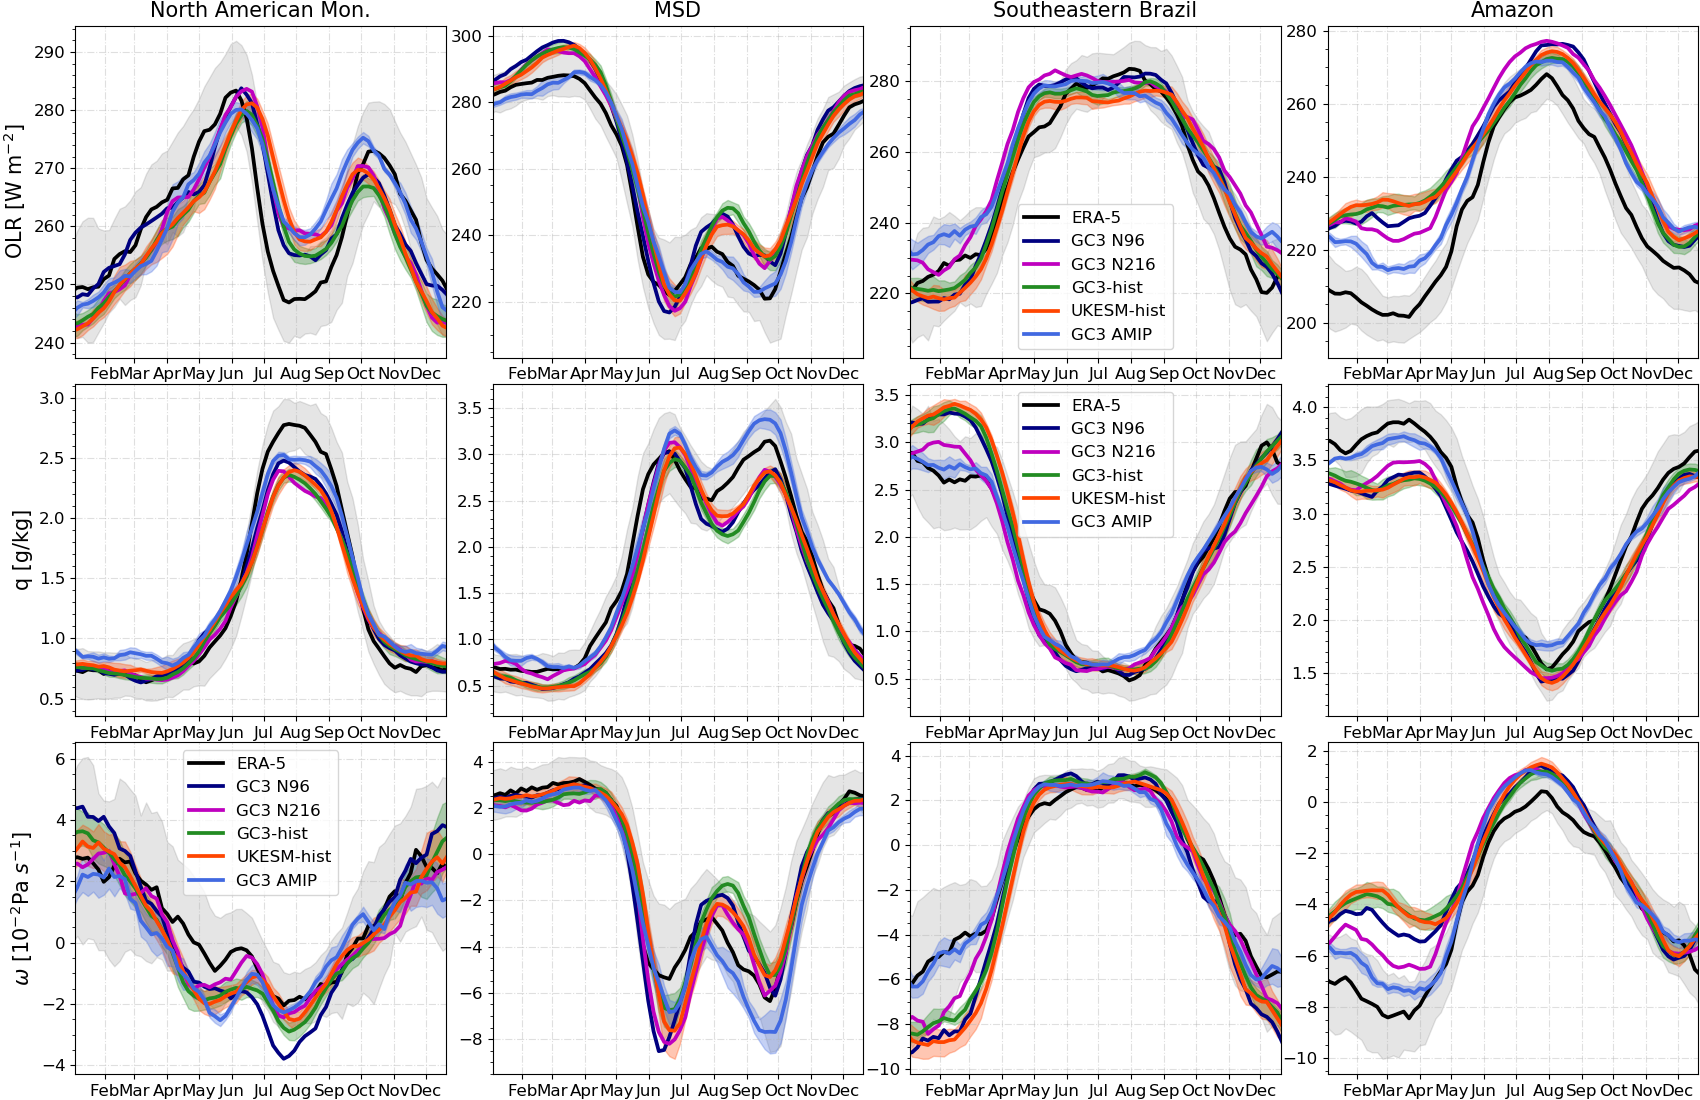
\includegraphics[width=\linewidth]{figures/fig9b.png}
\caption[Seasonal cycle of measures of convection in the AMS]{Pentad-mean (upper) outgoing long-wave radiation (OLR), (middle) specific humidity at 500-hPa and (lower) $\omega$ 500-hPa. These are shown from left to right for the North American Monsoon, the Midsummer drought, southeastern Brazil and the core Amazon. The uncertainty in ERA-5 data, shown as faint gray shading was estimating by bootstrapping with replacement the ERA-5 record 10,000 times. }
\label{fig:9}
\end{figure}

In the MSD region, OLR and $q$ show signs of convective activity from mid-April, as OLR sharply decreases and moisture increases.
%The key characteristic of the MSD is the modest decrease in rainfall in the midsummer.
The characteristic MSD bimodal distribution of precipitation can also be observed as two troughs of OLR, and $\omega$ and two peaks in $q$ separated by a period of relatively higher OLR, lower $q$ and weaker ascent from June 15 until late August.
%The reanalysis data shows that during the MSD period OLR increases by 10 W m$^{-2}$, $\omega$ decreases by 0.015 Pa s$^{-1}$ and $q$ decreases by 0.5 g/kg.
Although arguably with a small dry bias with shallower convection after mid-July, the simulations follow closely the observed seasonal cycle.

The simulated conditions during the first peak period show similar OLR and mid-level moisture but stronger ascending motions, which may explain the positive rainfall bias in this period (Fig. \ref{fig:8}a).
In the period between the first peak and the MSD, the simulated OLR increases more sharply than observations from 220 W m$^{-2}$ (June 15) to 250 W m$^{-2}$ (early August), with similar behaviour in $\omega$ and $q$, which may also be related to the strong variations of precipitation within the rainy season in the simulations. 
%In the same period, the simulated moisture and ascent decrease more sharply than observations, in agreement with the stronger variations of precipitation (Figure \ref{fig:8}a).
%The stronger than observed changes to the characteristics of convection are consistent with the sharper than observed midsummer drought in the simulations showed in Figure \ref{fig:8}a.
The period during the second peak of rainfall in September shows signs of shallower convection and a drier mid-level when compared to ERA5.
%The characteristics of the retreat stage of rainfall at the start of October shows close agreement between reanalysis and simulations.
%Overall, the models seem to reproduce the annual cycle of OLR and

In southeastern Brazil, the simulations reasonably follow the timings of the annual cycle of OLR, $q$ and $\omega$ of the reanalysis, particularly during austral winter. The moisture $q$ in ERA5 during  the dry seasons of austral fall, winter and spring is reasonably simulated by all the experiments. However, during austral summer, the coupled model simulations show significant biases characterised by stronger ascent and increased specific humidity in the mid-levels, although the height of convection (OLR~ 225 W m$^{-2}$) is only modestly higher in the simulations.

%The seasonal cycle of these proxies for convective activity in the Amazon basin are shown by Figure \ref{fig:8}.
The simulated OLR, q and $\omega$ exhibit the highest biases in the Amazon. During austral summer, particularly January and February, the simulated convective activity is shallower (OLR bias of +25 W m$^{-2}$) and weaker (positive $\omega$ bias +0.02 Pa s$^{-1}$) and the mid-level troposphere is drier (~-0.5 g/kg) than in ERA5. All these biases are in agreement with the dry Amazon bias described in the previous section. Despite biases in the magnitude of OLR, $q$ and $\omega$ during peak convective activity, the seasonal variation is very well simulated so that convective activity, as evidenced by these metrics, starts and ends in the simulations within one or two pentads of the reanalysis. 

The smallest biases in the coupled simulations are those of GC3 N216-pi, for all the regions.  The simulated OLR, $q$ and $\omega$ in GC3-amip in southeastern Brazil and the Amazon show a much better agreement with the reanalysis during austral summer than the rest of the simulations.
This section shows that while precipitation may be well represented in a region, e.g., the North American monsoon, competing model biases in the strength of convection and moisture may lead to a right representation of precipitation. 


\section{ENSO Impacts}\label{sq:enso1}

El Ni\~no-Southern Oscillation (ENSO) teleconnections are the prominent source of interannual variability for the AMS \citep{vera2006}, as summarized in section \ref{sub:lit_enso}.
The response to ENSO events in UKESM1 and HadGEM3 is investigated in this section, first by investigating the mean response to ENSO events and then by analysing possible sources of non-linear teleconnections.

%Throughout this section, ENSO events were defined when the DJF-mean Ni\~no 3.4 index was above or below 0.65 \citep{trenberth1997}.   



\subsection{Canonical impacts to the AMS}

\begin{figure}[t!]
\centering
 %\noindent
 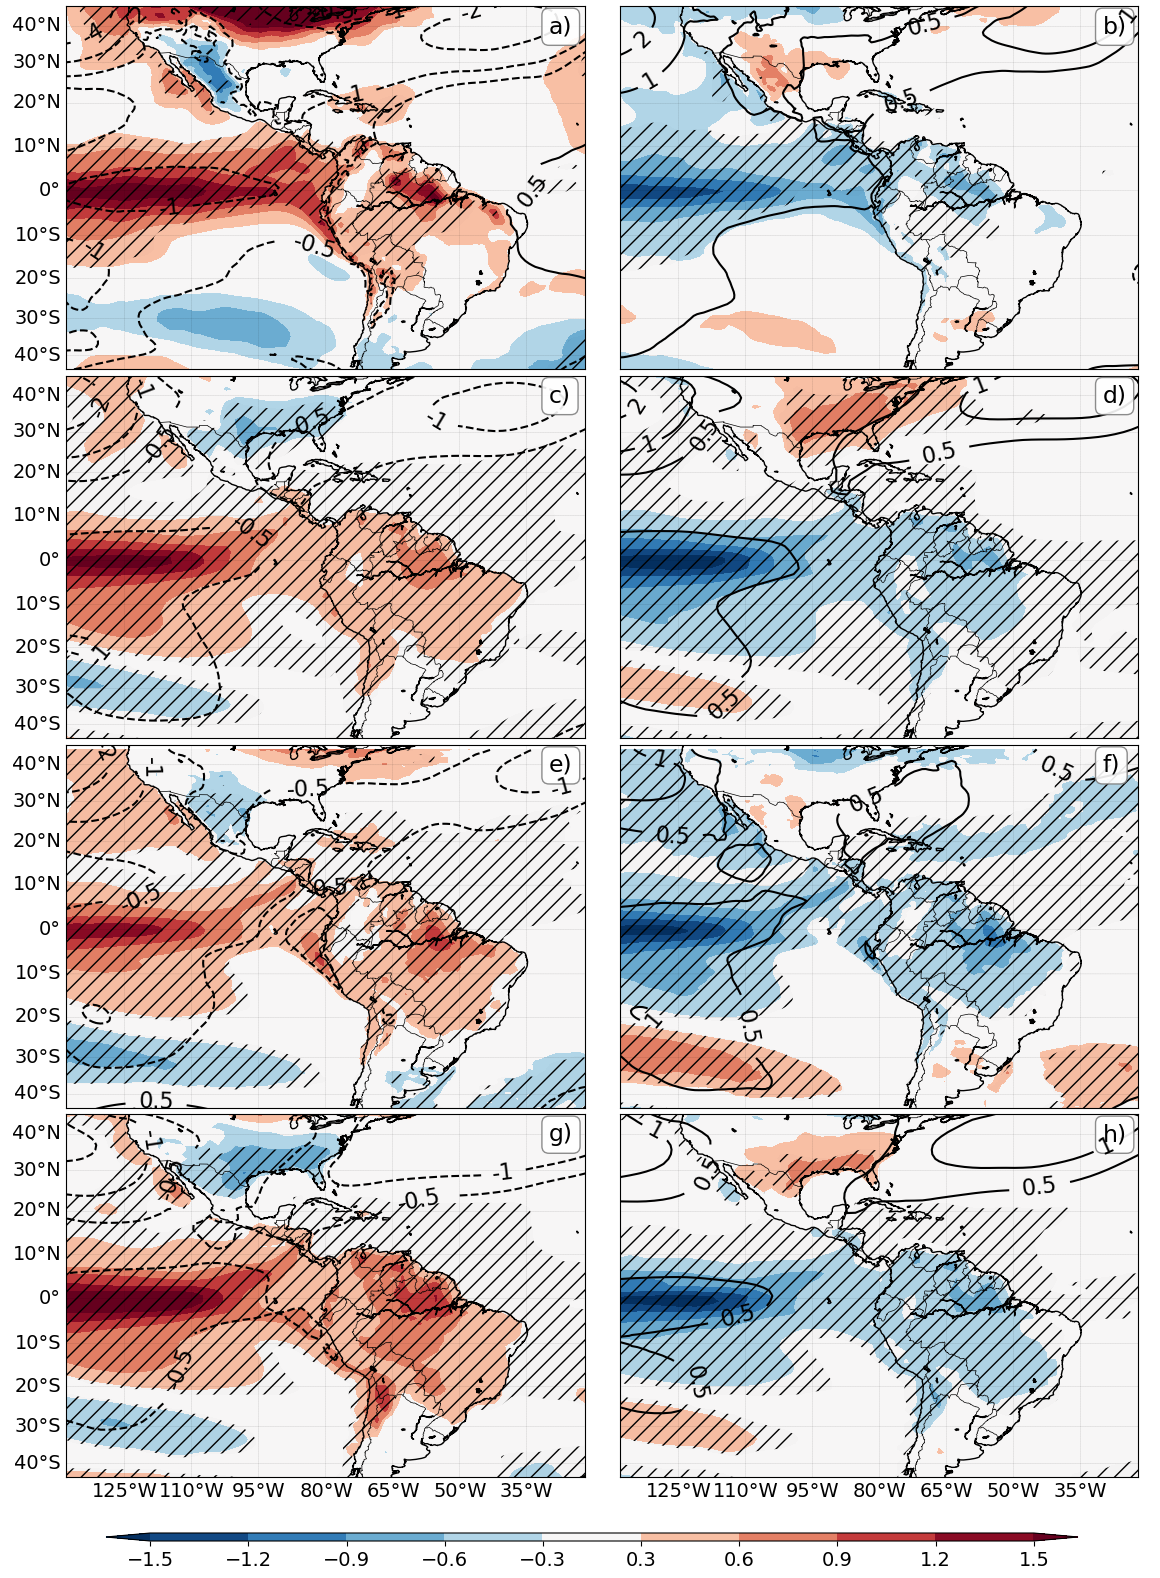
\includegraphics[width=0.81\linewidth]{figures/ensotemp_3}
\caption[ENSO teleconnections of temperature and SLP to the region of the AMS]{ DJF Temperature anomalies (colour contours in K) and SLP (line contours in hPa) during (a, c, e, g) El Ni\~no and (b, d, f, h) La Ni\~na events. Results are shown for (a, b) ERA-5, (c, d) UKESM1-hist, (e, f) GC3 N96-pi and (g, h) GC3 N216-pi. The hatched regions denote differences between ENSO phases and the climatological state with significance to the 99\% confidence level from a Welch t-test for the temperature field. }
\label{fig:10}
\end{figure}

The surface temperature and sea-level pressure (SLP) responses to ENSO events are shown in Figure \ref{fig:10} for HadGEM3, UKESM1 and ERA5 data during DJF, the season of strongest impact of ENSO events.
The characteristic warm anomaly during El Ni\~no events in the East Pacific Ocean does not extend as far east in the simulations as in the HadSST dataset or ERA5. In turn, the cold anomalies during La Ni\~na events in the Central Pacific are colder in the simulations than in ERA5. 
The impact to southern North America, i.e., colder (warmer) conditions in southern (northern) North America during El Ni\~no events is relatively well simulated. For example, the simulated and observed impacts to South America, e.g., the cold anomalies during La Ni\~na events in northern South America are well simulated. However, the low resolution simulations show a broader and stronger than observed negative response in southeastern US to El Ni\~no events. 

%The simulated teleconnection pattern to North America is better represented in GC3 N216-pi. % It is worth noting that the medium resolution simulations seems to simulate stronger El 

\begin{figure}[t!]
\centering
 %\noindent
 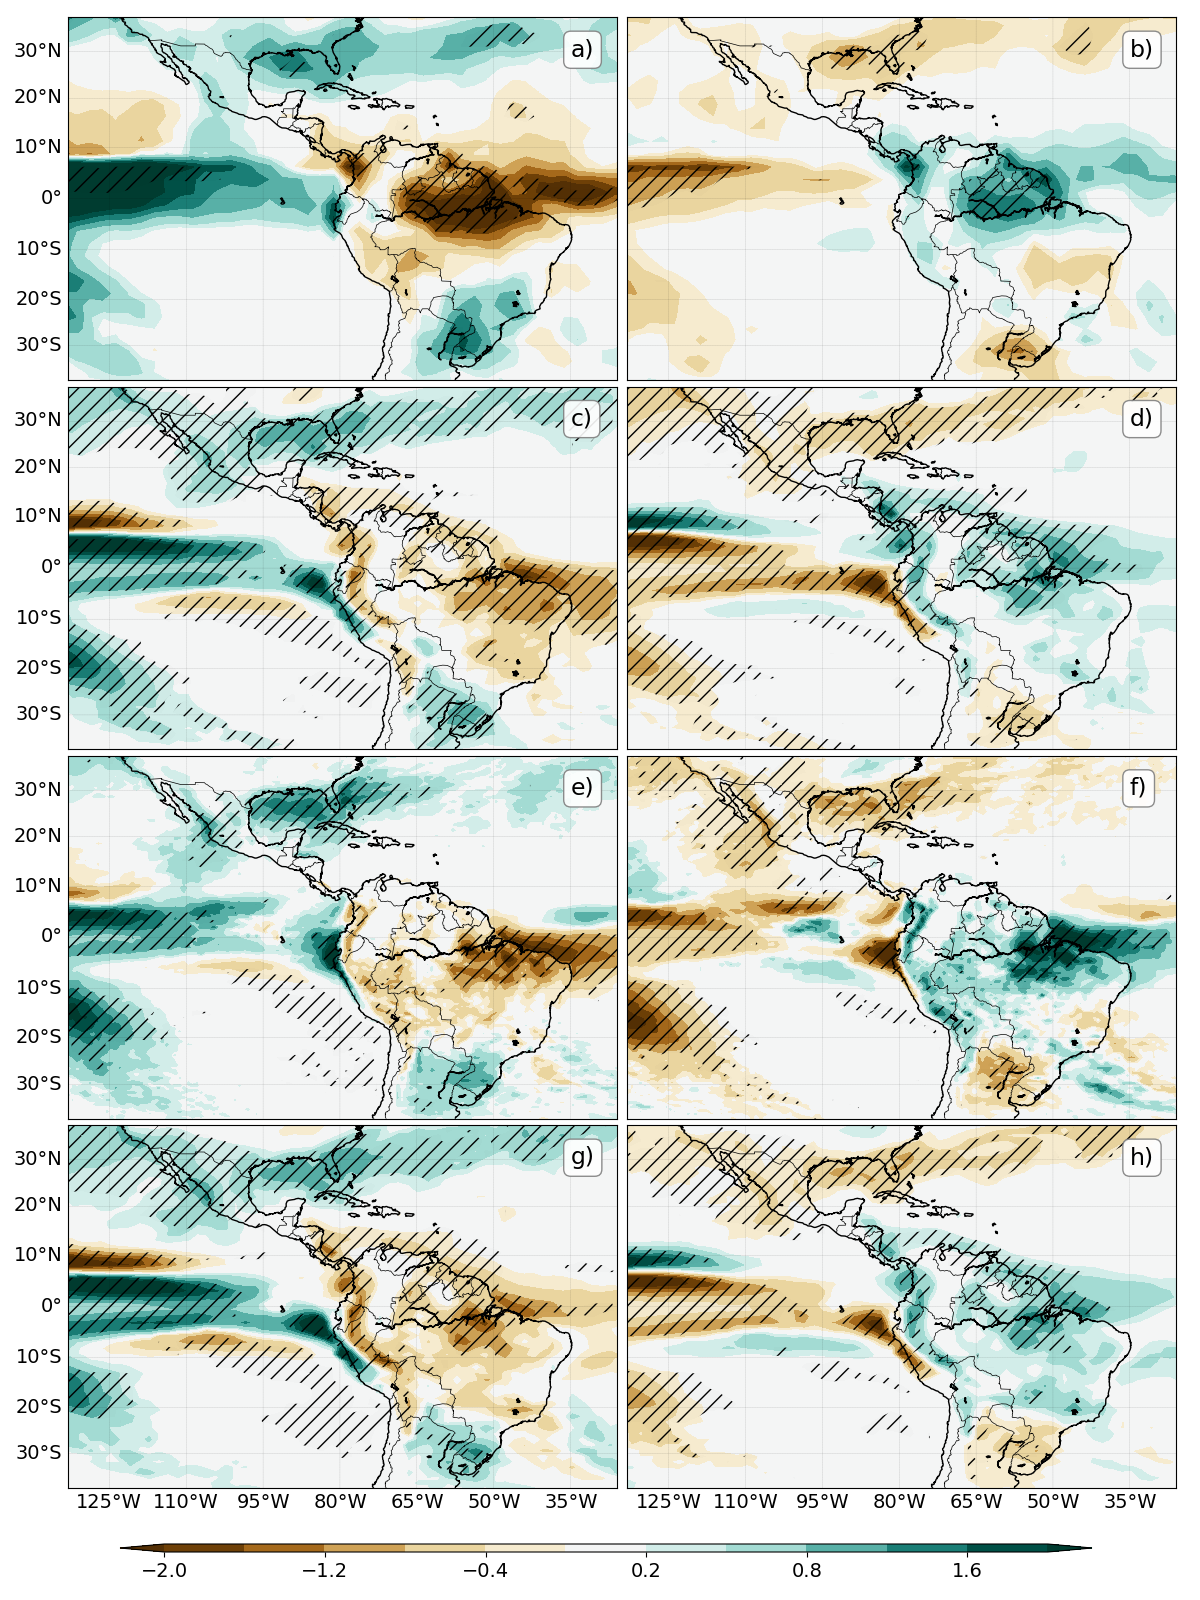
\includegraphics[width=0.81\linewidth]{figures/ensopr_3}
 \caption[ENSO precipitation teleconnections to the AMS]{As in Figure \ref{fig:10} but for the rainfall response [mm day$^{-1}$] using GPCP as the observational dataset.}
%\caption{ Precipitation  DJF response to (a, c, e, g) El Ni\~no and (b, d, f, h) La Ni\~na events in (a, b) GPCP, (c, d) UKESM1, (e, f) GC3.1 N96 and (g, h) GC3.1 N216. The hatched regions denote 99\% significance from a Welch t-test. }
\label{fig:11}
\end{figure}

The SLP response in the north Pacific and North America, known as the Pacific North-American pattern (PNA), is linked with a displacement of the subtropical jet affecting the eastward propagation of wave activity that reaches the North Atlantic  \citep[e.g.][]{bayr2019,jimenezesteve2020}.
During  El Ni\~no events, the Aleutian Low is strengthened in ERA5, with a strong SLP anomaly (-4 hPa) off the coast of California. The models show a similar but smaller SLP response in the same region.  El Ni\~no events events are associated with a negative phase of the North Atlantic Oscillation (NAO), with an opposite response for La Ni\~na events \citep{fereday2020}. While the models seem to be able to capture this response of the NAO, the simulated response is weaker than observed.  \added{ A sensible representation of the ENSO-PNA tropospheric teleconnection is important to  fully simulate ENSO impacts to North America \citep{bayr2019} and northeast Brazil \citep{hastenrath2006,taschetto2016}.  }




\begin{figure}
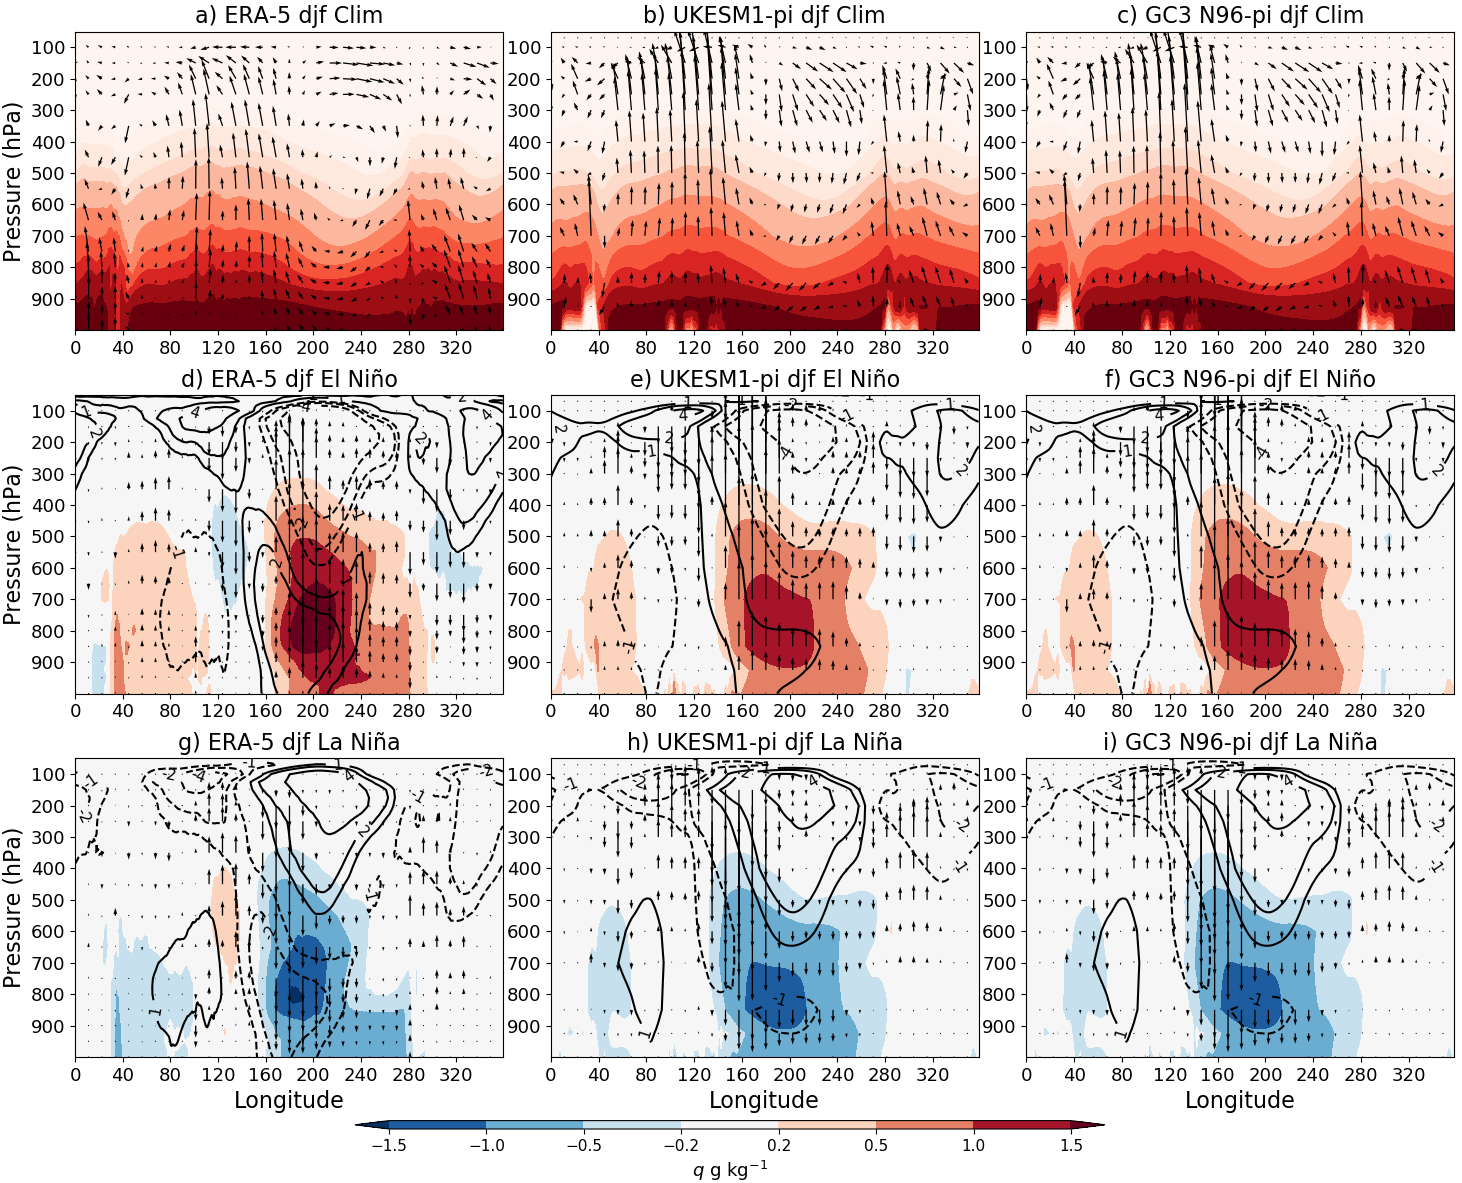
\includegraphics[width=\linewidth]{figures/walkerfinal}
\caption[Walker circulation anomalies associated with ENSO]{DJF Longitude-height Walker circulation \added{(a-c) climatologies and (d-i) anomalies of specific humidity (colour-contours), $\omega$ (vectors) and zonal wind (line-contours) during (d-f) El Niño events  and (g-i) La Niña events. Results are shown for ERA-5 (left), UKESM-pi (middle) and HadGEM3 N96-pi (right)}.}
\label{fig:swalker}
\end{figure}


The rainfall anomalies associated with ENSO events (Figure \ref{fig:11}) show that three regions in the AMS have a significant precipitation response.
In southern North America, rainfall increases (decreases) during El Ni\~no (La Ni\~na) events due to the effects of the PNA pattern on the subtropical jet, which influences the frequency and latitude of propagation of wintertime midlatitude disturbances which are the main source of rainfall in the region during the dry season \citep{vera2006,bayr2019}.

The GPCP dataset (Figure \ref{fig:11}a, b) shows significant boreal winter rainfall increases in southeastern US and the Gulf of Mexico during El Ni\~no events, and an opposite response to La Ni\~na phases. All the simulations reproduce this impact pattern. 
The models also simulate the observed response in South-Eastern South America (SESA) of positive anomalies during El Ni\~no and negative anomalies during La Ni\~na events. \added{This impact to SESA is due to the subsidence induced by the anomalous Walker circulation which modifies the moisture transport by the SALLJ from the Amazon to SESA \citep{montini2019}.}

The anomalies in the Amazon show the strongest response to ENSO events in the observations. Significant positive (negative) rainfall anomalies during the negative (positive) phase of ENSO in northern South America are observed in GPCP. All the simulations show a very similar and statistically significant response.\added{ This teleconnection is due to the coupling of ENSO with the Walker circulation \citep{vera2006,cai2019pantropical}, which is illustrated in Figure \ref{fig:swalker}, and the effect of the ENSO-PNA telecconection in the tropical north Atlantic.  }

\begin{figure}[t!]
\centering
 %\noindent
 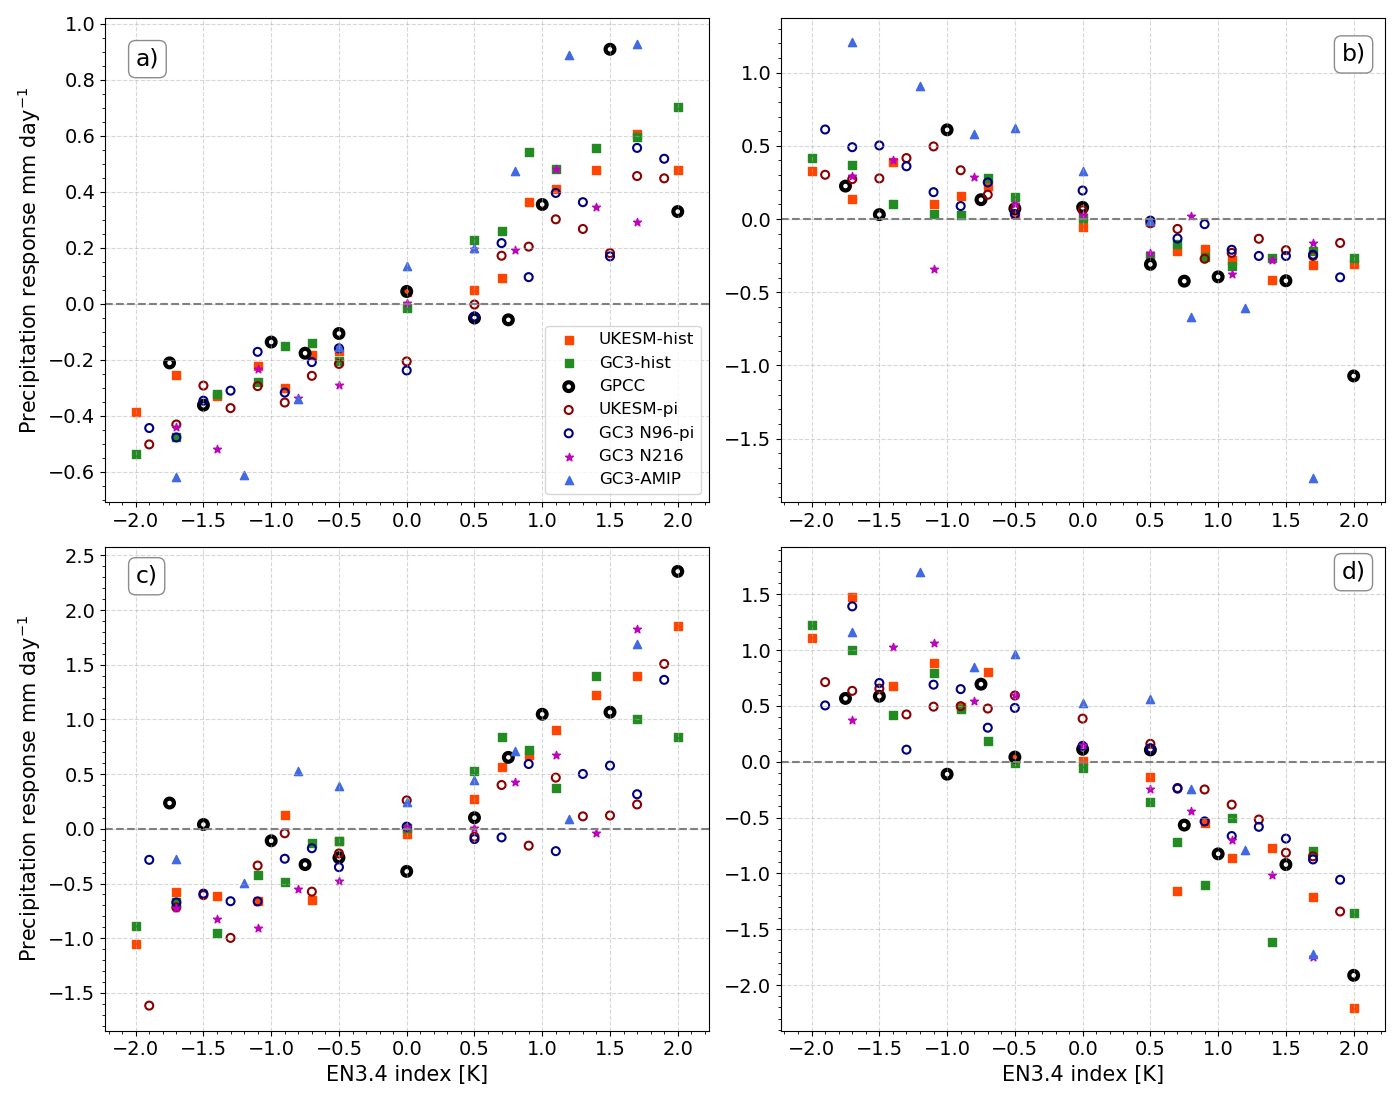
\includegraphics[width=\linewidth]{figures/fig_ensolinear}
\caption[Linearity of the precipitation response to ENSO events]{Precipitation response [mm day$^{-1}$] as a function of the El Ni\~no 3.4 index (see text) for (a) southwestern North America [20-37$^\circ$N, 112-98$^\circ$W], (b) Central America and southern Mexico [5-19$^\circ$N, 95-83$^\circ$W],, (c) Sout-Eastern South America [35-25$^\circ$S, 60-50$^\circ$W], and (d) the Amazon [10-0$^\circ$S, 70-45$^\circ$W]. The observation scatter points are from GPCC in the period of 1940-2013.}
\label{fig:12}
\end{figure}

The climatological Walker circulation during DJF shows strong ascent in the 100-160$^\circ$E and the 280-310$^\circ$E regions (Figure \ref{fig:swalker}a), which correspond to the maritime continent and South America, respectively. During El Ni\~no events, there is increased specific humidity throughout the lower troposphere in the Central and Eastern Pacific, associated with ascending motions in this region and negative low-level wind anomalies and positive upper-level wind anomalies (Figure \ref{fig:swalker}d). In other words, an eastward shift of the Walker circulation. The wind, vertical velocity and specific humidity anomalies are the opposite during La Niña events, indicative of a stronger Walker circulation shifted west. 
The models seems to broadly reproduce the observed changes to the Walker circulation during ENSO events (Figure \ref{fig:swalker}).

\added{The anomalous descent over equatorial South America is one cause for the drying response seen during El Niño in the Amazon \citep{marengo2012,cai2020}. However, 
the ENSO-PNA teleconnection decreases in the tropical north Atlantic (Fig. \ref{fig:10}), inducing a warming of the SSTs and a delay in the southward migration of the Atlantic ITCZ \citep{andreoli2012seasonal,jimenez2021}. Even though the models are able to simulate the ENSO-PNA SLP effect, this effect is slighlty weaker than observed, particularly for El Niño events.}

 Figure \ref{fig:12} shows the observed and simulated precipitation responses in four regions of the AMS binned by the magnitude of ENSO events, measured by the EN3.4 index. This figure aims to show  the degree of linearity of ENSO teleconnections to the AMS, i.e., a precipitation response that linearly scales with the magitude of the ENSO event.
 \added{Both simulated and observed responses show degrees of non-linearity in various regions. For example, the precipitation response in the Amazon to La Niña events in observations appears to be relatively constant regardless of the strength of the event whereas in GC3 N96-pi the strongest La Niña events do not produce the strongest precipitation response over this region. This evidence suggests that for some regions there are varying degrees of non-linearity of ENSO impacts.}
%While the observed response shows some degree of linearity for El Ni\~no events in South America (panel d), the majority of the observed responses, particularly to La Ni\~na phases, are not linear. However, the simulations show several signs of linearity. For instance, consider the historical experiments, which show that the precipitation responses in southwestern North America, SESA and the Amazon increases roughly linearly as the magnitude of SST anomaly increases. In contrast, some other simulated responses, e.g. to La Ni\~na phases in South America in the piControl simulations, show signs of non-linearity.



\subsection{The role of ENSO flavours}
  
\begin{figure}[t!]
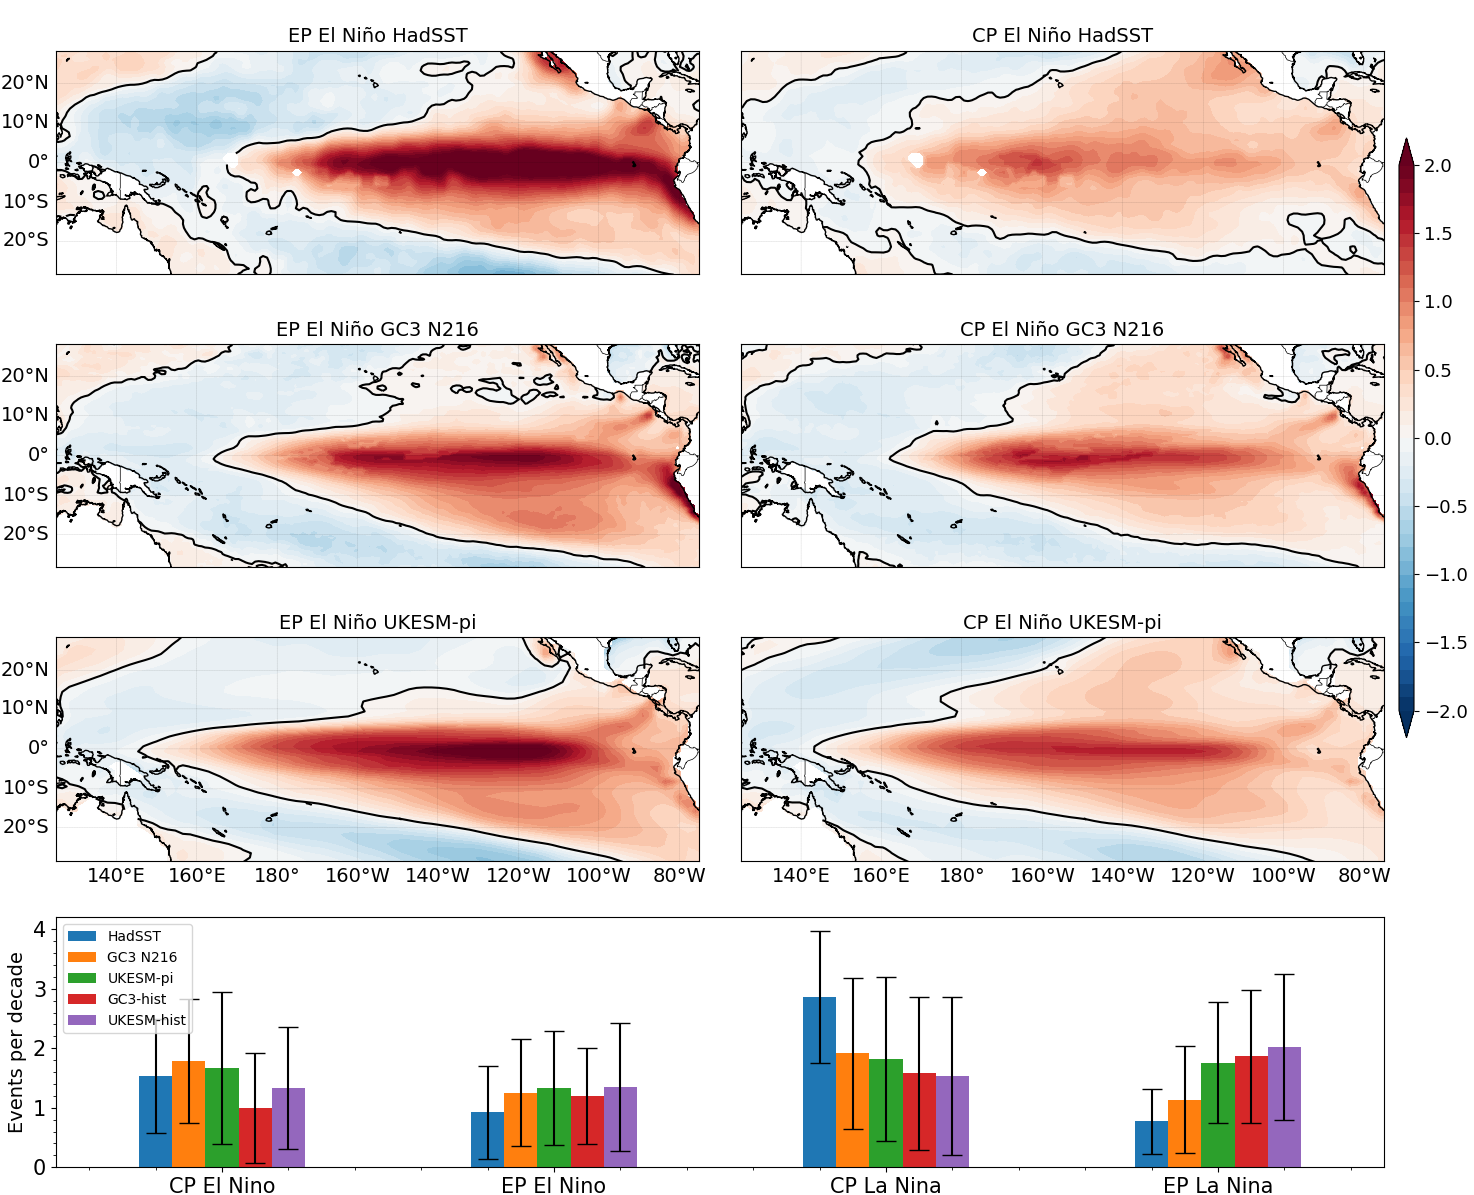
\includegraphics[width=\linewidth]{figures/epcpmap}
\caption[Diversity of ENSO SST patterns]{SST anomalies [K] for East Pacific (EP) and Central Pacific El Niño events in HadSST, GC3 N216 and UKESM piControl.  In the bottom panel, the frequency of events per decade (with standard deviation as error bar) is shown for HadSST and the simulations used in this study.
}
\label{fig:s1}
\end{figure}


  
As described in section \ref{sub:lit_enso}, not all ENSO events are observed with the same SST  pattern in the Pacific Ocean. These different SST patterns are considered to be a source of non-linearity of ENSO impacts over South America \citep{sulca2018,cai2020}.
Figure \ref{fig:s1} shows that both UKESM1 and GC3 reasonably simulate the observed SST patterns associated with EP and CP El Niño events, although the CP SST patterns in the simulations spread further to the east than the HadSST dataset.
The simulations are also able to replicate very broadly the observed differences in the frequency of each event as CP La Niña events are more frequent than EP La Niña events, while the opposite is true for El Niño events.

Furthermore, Figure \ref{fig:senso} compares the precipitation anomalies for each type of ENSO event in observations with three simulations: GC3 N96-pi, GC3 N216-pi and GC3-amip. 
%The observations show significant precipitation responses differences in the Amazon, the Brazilian Nordeste and SESA between CP and EP events; however, these differences are less obvious in the coupled simulations (GC3 N96-pi, GC3 N216), but not in GC3 AMIP.
The observed precipitation response in the GPCC dataset to EP La Niña over equatorial South America is not significant and is smaller than the strong positive response to CP La Niña events in the same region. However,  the simulated response in GC3 N96-pi and GC3 N216 during La Niña events appears to be more independent of the type of event. In contrast, the GC3-amip simulations shows different magnitudes of responses to different types of La Niña events, in particular a positive, and significant, anomaly for CP La Niña events in the Amazon and weaker but not significant anomalies during EP events, which agrees with observations.

\begin{figure}[t!]
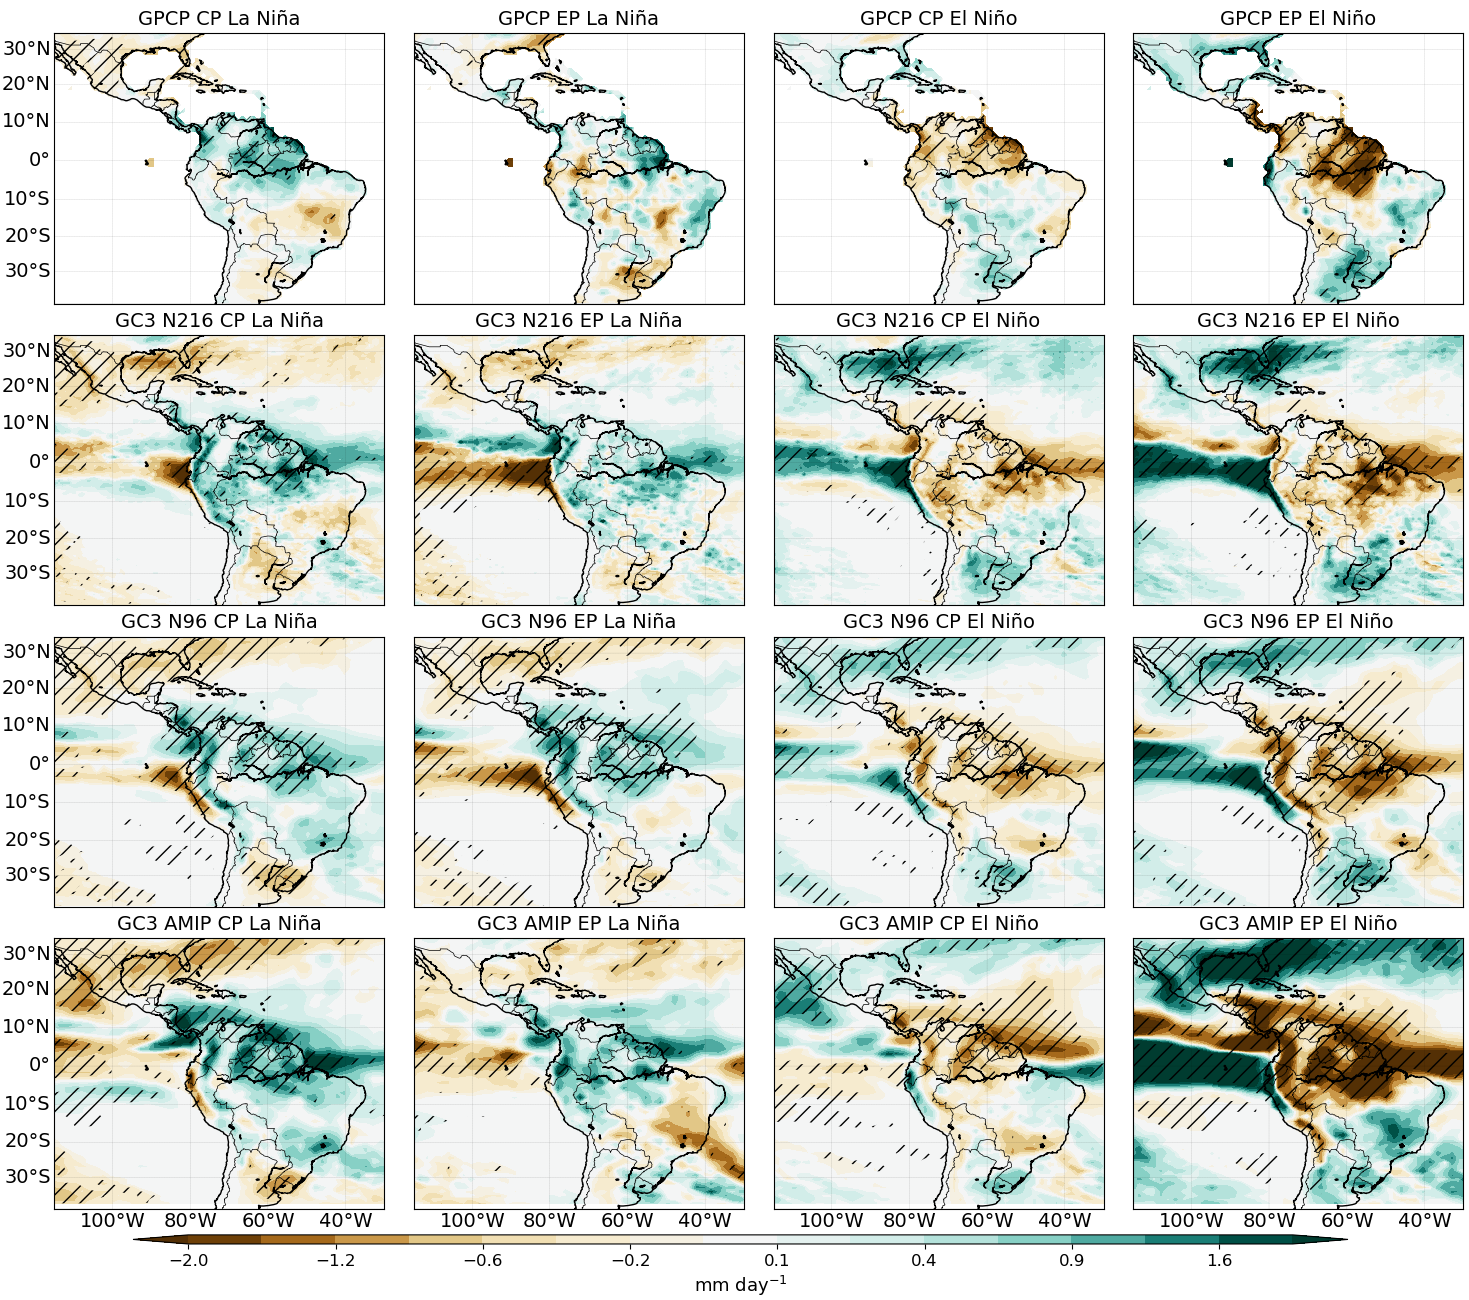
\includegraphics[width=\linewidth]{figures/cppranomalies_ff}
\caption[Precipitation anomalies to different ENSO flavours]{Precipitation anomalies in GPCC 1940-2013, GC3 N216-pi, GC3 N96-pi and GC3 AMIP for the four different types of ENSO events, as defined by \cite{cai2020}. Statistically significant anomalies (95\% confidence level) are hatched.}
\label{fig:senso}
\end{figure}  

 The observed response to El Niño events in GPCC is also dependent on the type of event. EP EL Niño events show significant negative anomalies over the Amazon and positive anomalies over SESA whereas CP events only show significant anomalies (-1 mm day$^{-1}$) over northeastern South America. While the coupled models (GC3 N96-pi and GC3 N216) show a stronger response to EP  EL Niño events than to CP events.
  In contrast, the response in GC3-amip agrees with observations, as stronger negative responses to EP El Niño events are observed in the Amazon compared to CP events in which the response is much weaker and is only significant in northeastern South America. In other words, GC3-amip agrees well with the observed non-linear impacts whereas the teleconnections in the coupled models do not seem to depend so strongly on the type of ENSO event.    

\subsection{A possible influence of the QBO on tropical ENSO teleconnections}

\begin{figure}[b!]
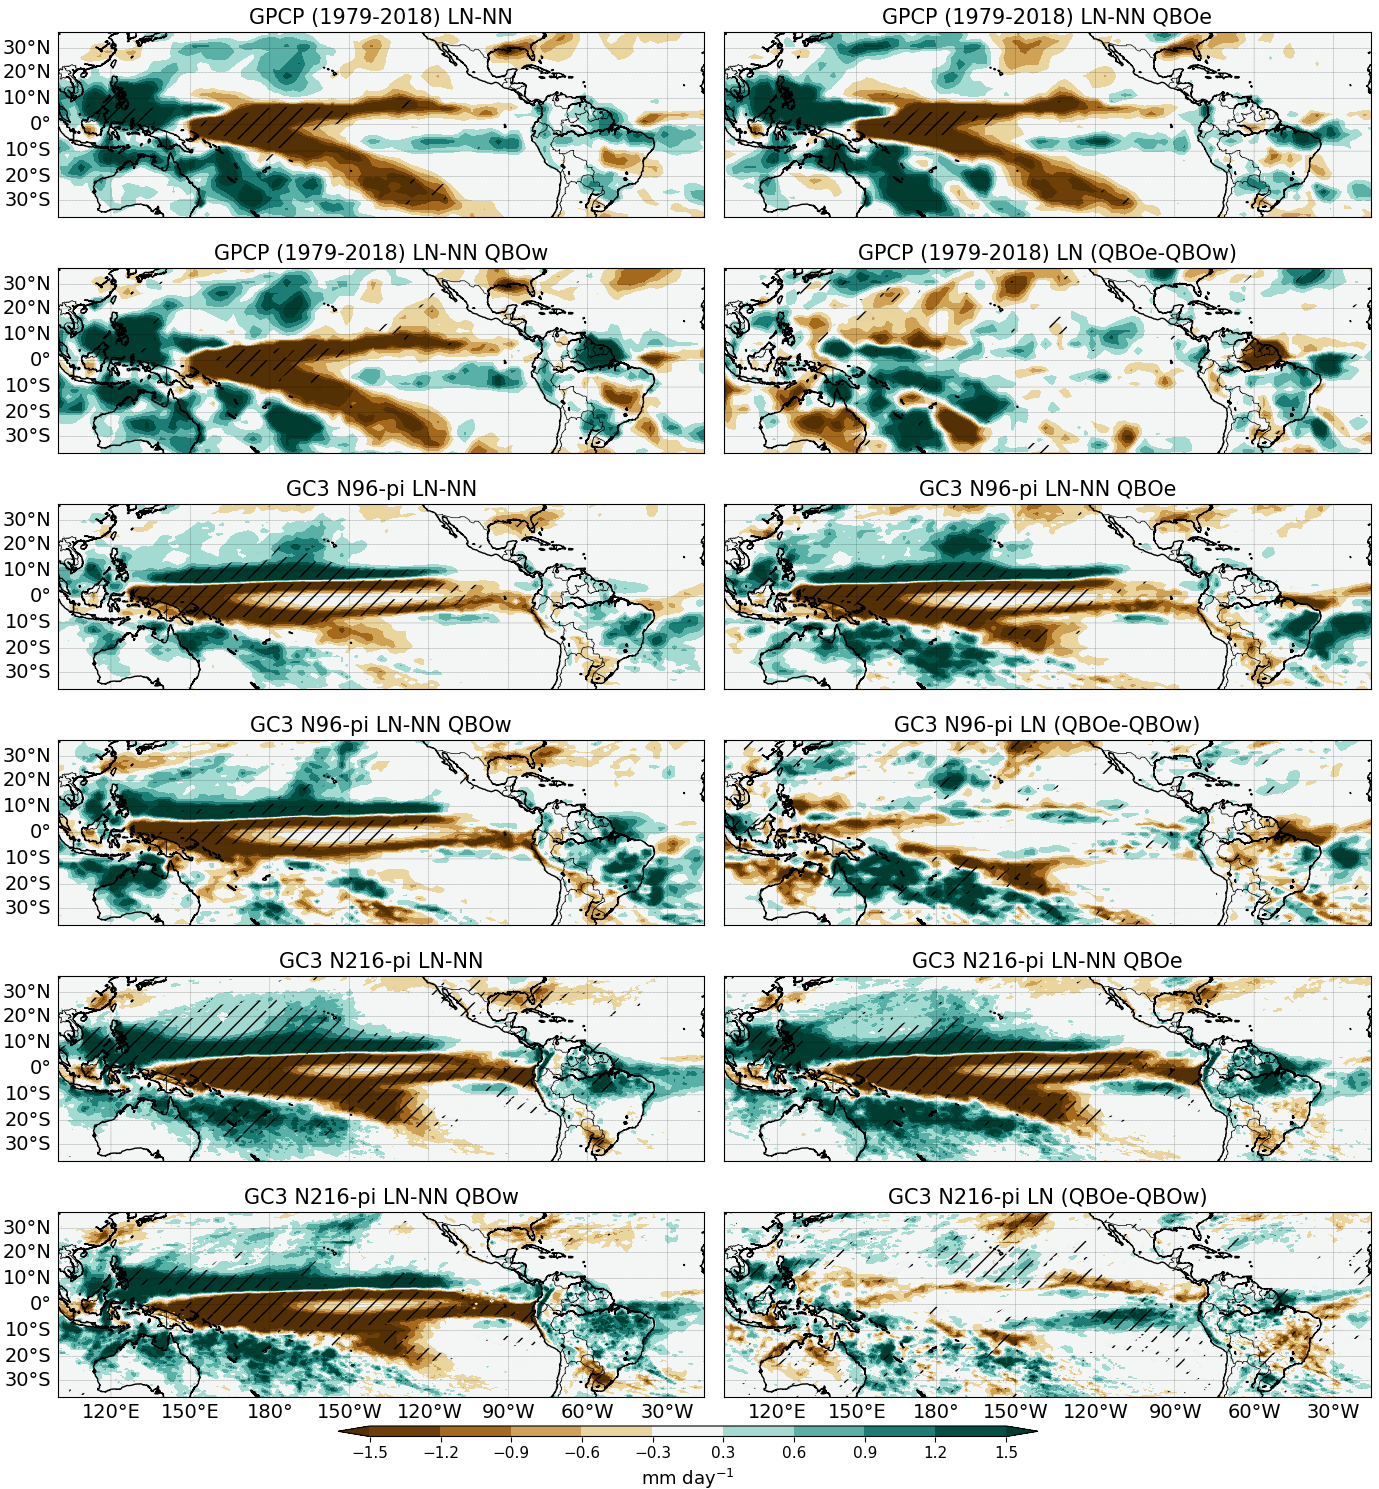
\includegraphics[width=\linewidth]{figures/trops_qbolnprfma}
\caption[Precipitation anomalies as a function of QBO and ENSO phases]{Composite precipitation differences during JFMA in GPCP (1979-2018), GC3 N216-pi and GC3 N96-pi between (top) La Niña and Neutral ENSO conditions. The two middle panels show a subset of the top panel, by separating the La Niña composite based on the phase of the QBO. The lower panel shows the differences QBO E-W during La Niña periods. Statistically significant anomalies (95\% confidence level) are hatched.}
\label{fig:qbopr_pis}
\end{figure}  

Section \ref{sq:qbolit} discusses the observational and modelling evidence that suggest a role for  the stratospheric quasi-biennial oscillation (QBO) in modulating the determine interannual variability of the Walker circulation and monsoons \citep{giorgetta1999,collimore2003,liess2012}. 
This section evaluates whether the simulations analysed in this chapter, as well as observations, show signs of an influence of the QBO on the AMS. 
In particular, the analysis aims to understand whether the QBO may be a source of non-linearity for the teleconnections of ENSO associated with deep convection and the Walker circulation. %In all cases, the phases of the QBO were defined using a 70 hPa zonal mean zonal wind index, with a threshold of +2 m s$^{-1}$ for the westerly phase (QBOw) and -2 m s$^{-1}$ for the easterly phase (QBOe).

\begin{figure}[b!]
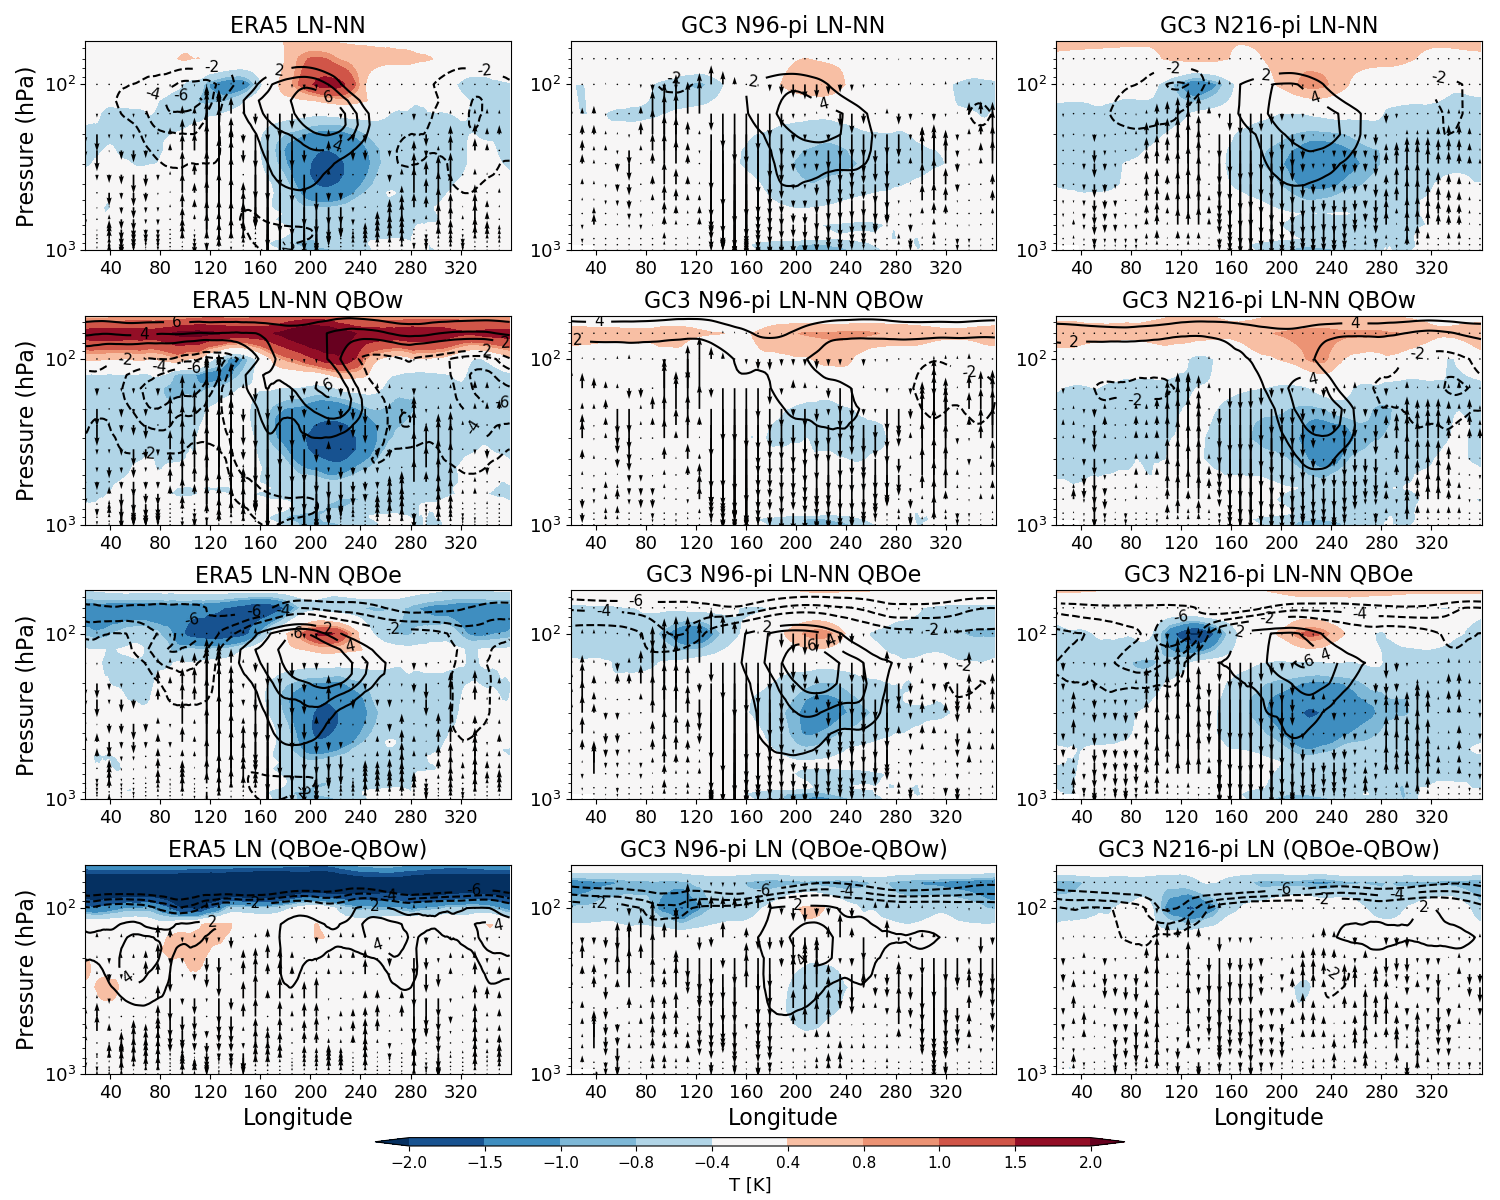
\includegraphics[width=\linewidth]{figures/walker_wqbo_jfma}
\caption[Walker circulation responses to La Niña under different QBO phases] {Longitude-height differences (JFMA) of equatorial (10S-10N) air temperature (color shading), zonal wind (contours) and vertical velocity ($\omega$ - vectors). The differences shown from top to bottom are between all La Niña (LN) periods and Neutral conditions (NN), between LN and NN during QBOw, LN-NN during QBOe, and the difference between LN events on different QBO phases (LN QBOe-QBOw). 
}
\label{fig:qbowalker_pis}
\end{figure}

Composites of the precipitation response to La Niña (LN) events in Figure \ref{fig:qbopr_pis} show that the phase of the QBO may determine the strength and location of the impact. 
While the precipitation difference in the western Pacific is relatively similar during QBOe than during QBOw in observations and simulations, the teleconnections to Australia, South America and the maritime continent are notably different depending on the QBO phase. 
In the GPCP dataset, the composite difference QBOe-QBOw during LN events suggests that the characteristic positive precipitation response during LN events in the Amazon, is largely associated with QBOw phases, whereas LN events during QBOe appear to have little effect over South America. 
A similar result is obtained for GC3 N96-pi. 

These precipitation responses are further investigated by changes in the overturning circulation (Figure \ref{fig:qbowalker_pis}). As depicted in Figure \ref{fig:swalker}, La Niña events are associated with a westward shift in the Walker circulation with a strenghtening of the low-level easterlies in the Pacific Ocean. 
Figure \ref{fig:qbowalker_pis} shows that during LN the tropical troposphere cools and the UTLS region in the Central Pacific warms. %These temperature anomalies are weaker in the simulations than in ERA5. 
The zonal wind anomalies in the upper-troposphere associated with LN events show different patterns and strengths during QBOw than during QBOe. The mean teleconnections during LN show positive zonal wind anomalies in the upper troposphere of the Pacific Ocean,  but these anomalies are stronger during QBOe than during QBOw in ERA5 and the two simulations shown. In ERA5, most of the upper troposphere shows positive zonal wind differences in the QBOe-QBOw panel. 

%There are three regions where ascending and descending motions are more greatly affected by LN events: the maritime continent, the Pacific Ocean and South America. The observed effect of the mean LN teleconnection is the following: anomalous ascent is seen in the maritime continent and in South America, in agreement with a stronger Walker circulation, whereas anomalous descending motions is observed in the Central and eastern Pacific associated with a westward shift of the Walker circulation. 

The effect of LN over ascending and descending motions is also affected by the QBO phase (Fig. \ref{fig:qbowalker_pis}). In ERA5 and the simulations, the anomalous ascent observed in South America during LN events is mostly associated with QBOw, whereas only small anomalous ascent is observed during QBOe. 
However, ERA5 disagrees with the simulations in the western Pacific region (140-180$^\circ$E), as the simulations suggest larger anomalous descent during QBOe than during QBOw, whereas in ERA5 these descending anomalies are larger during QBOw. 

The effect of the QBO during the positive and the neutral phases of ENSO were also evaluated but these results are not shown because, although tentative suggestions were found that the QBO may play a role during these other phases of ENSO, there was little agreement between the models and ERA5/observations. Model biases in the representation of the QBO, specially the temperature signal associated with circulation of the QBO, most clearly seen in the bottom panels of Figure \ref{fig:qbowalker_pis}, in addition to short record of the reanalysis evidence (ERA5) or presented in this chapter warrants both caution and future work. 
%This topic will be investigated in the next chapters.

\section{Summary and discussion}



 This chapter assessed the contributions to CMIP6 from the models HadGEM3 and UKESM1 for their representation of the AMS climate and associated large-scale tropical circulation. These CMIP6 experiments allow the comparison of the effect of including Earth System processes or increasing resolution for representing regional monsoon rainfall. 
A schematic in Figure \ref{fig:13} shows the primary components of the AMS climate and summarises the main biases found in these simulations and this chapter.
%The study focuses on four regions in the AMS domain, the North American Monsoon, the MSD region of southern Mexico and Central America, southeastern Brazil and the Amazon.



Rainfall in the North American Monsoon was particularly well simulated by the models. The seasonal cycle, peak monsoon rainfall rates and timings of monsoon onset and retreat in the simulations agreed well with TRMM. The historical experiments overestimate the mean temperature in most of the Americas by 1.5 K, but particularly in boreal summer in southwestern North America (+4 K). Despite this warm bias, the seasonal cycles of precipitation and surface temperature are well represented by these models.  These results suggest model improvement of the simulation of the North American Monsoon from previous versions of the MOHC models \citep{arritt2000}, and most of the model cohorts of CMIP3 and CMIP5 \citep{geil2013}. However, these models continue to show biases during monsoon retreat as rainfall does not decrease as sharply as in observations after mid-September, which suggests a continued bias in the winter-time precipitation associated with cold-fronts \citep{adams1997}. %Further research into the variability of the North American seasonality may be explored using these models given their skilfull representation of the seasonal cycle.

\begin{figure}[t!]
\centering
 %\noindent
 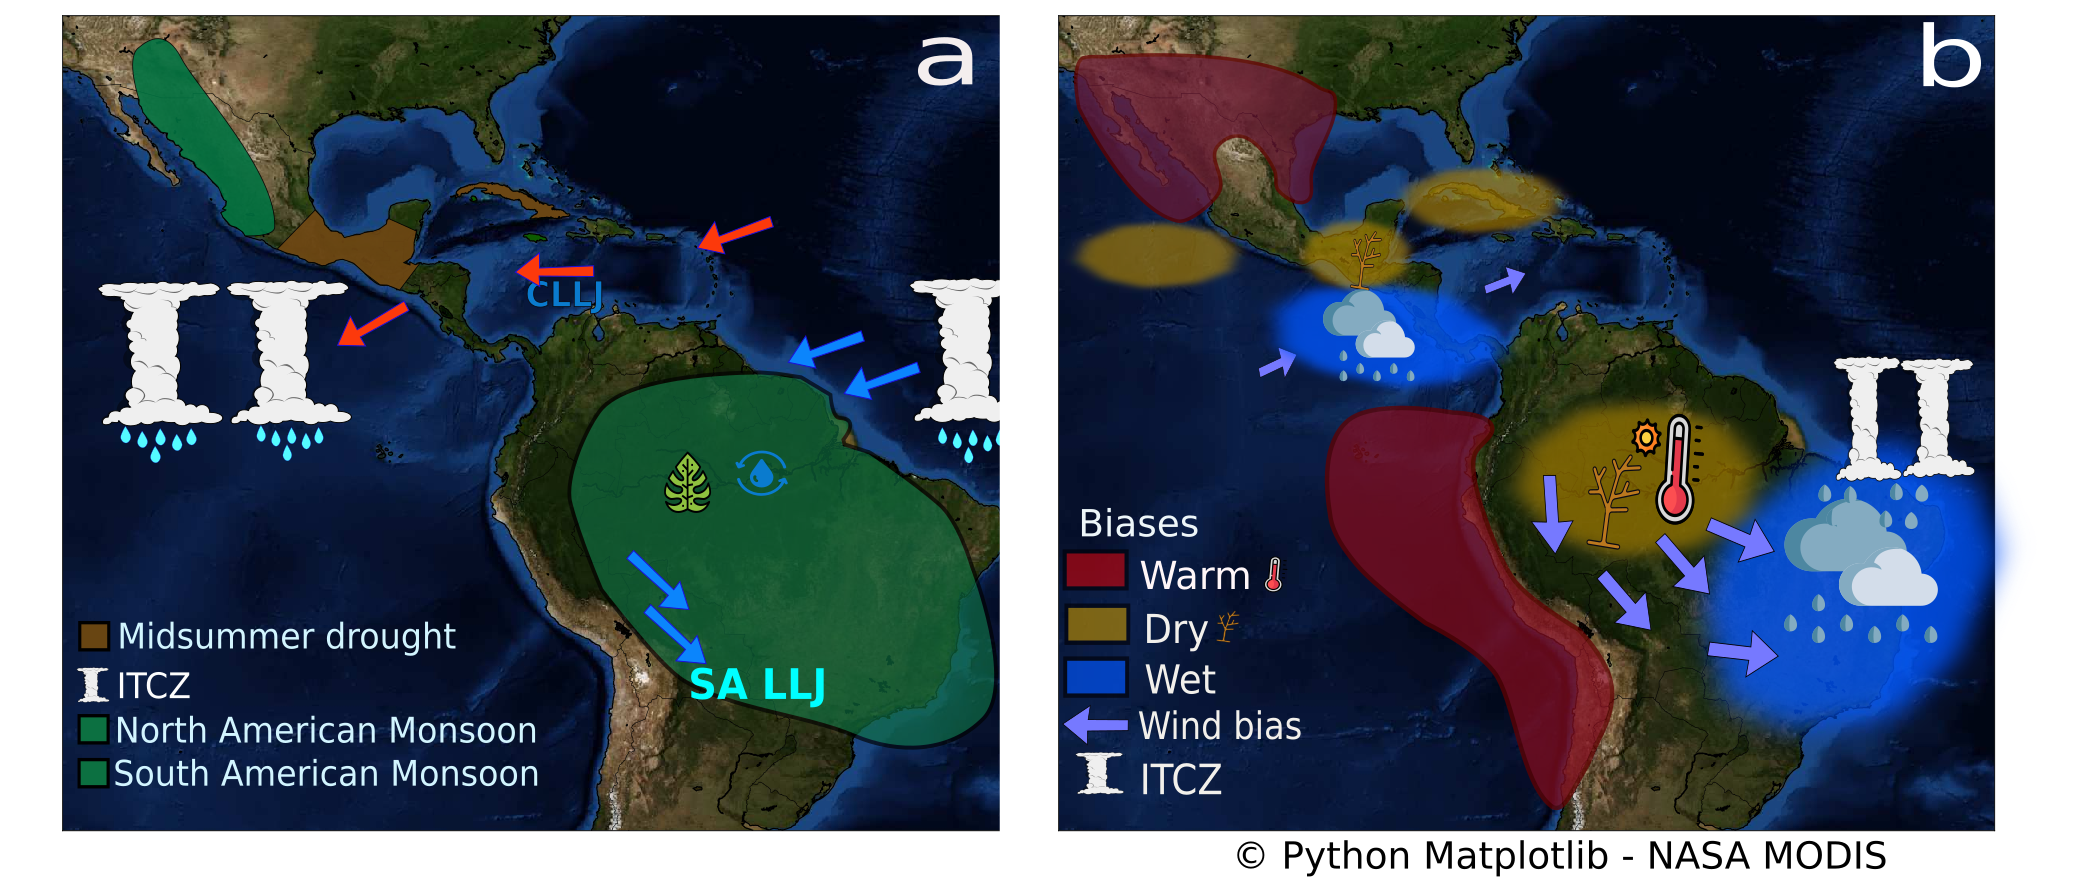
\includegraphics[width=\linewidth]{figures/drawing_e}
\caption[Summary schematic of biases in UKESM1 and HadGEM3]{Schematics of (a) the main features in the AMS and (b) the main biases in UKESM1 and HadGEM3. In (a) the boreal summer easterlies (red) and austral summer circulation (blue) are shown with the Caribbean and \added{South American} Low-level Jets (CLLJ and \added{SALLJ}, respectively). In (b) the biases are shown for the respective northern and southern Hemisphere summers. The ITCZ bias in (b) refers to the southward displacement bias of the Atlantic ITCZ in the simulations.  }
\label{fig:13}
\end{figure}

    The Midsummer Drought (MSD) of southern Mexico and Central America is a regional feature of precipitation that most CMIP5 models do not capture \citep{ryu2014}. 
The MSD in UKESM1 and HadGEM3 is relatively well represented. However, the experiments analysed in this chapter simulate a wetter-than-observed first peak of precipitation and a drier MSD period, therefore simulating a larger difference between the first peak and the dry period. %While in observations this difference  between the first peak and the MSD period ranges between 2-3 mm day$^{-1}$, in the simulations the difference is closer to 6 mm day$^{-1}$.
Rainfall during the first peak has been too wet in these models since CMIP3, suggesting a persistent wet bias in this region, likely associated with the bias in East Pacific ITCZ also shown in this chapter and in recent studies \citep{ryu2014,mulcahy2018}. 
In contrast, the so-called second peak of precipitation, observed in late August, is simulated in close agreement with TRMM, except in the GC3 AMIP experiment, which has a wet bias of 2 mm day$^{-1}$ at this stage. The relative skill of UKESM1 and HadGEM to simulate this bimodal regime of precipitation makes these simulations ideal to understand the mechanisms underpinning the MSD, an outstanding question (see Section \ref{sq:litmsd}).  


The East Pacific ITCZ migration and position is relatively well represented by the models (Figs. \ref{fig:3} and \ref{fig:4}). However, the models overestimate the boreal summer rainfall near the coast of Central America (Figure \ref{fig:8}). These biases are associated with an easterly wind bias at low levels, suggesting a bias in the flow from the Caribbean Sea into the Eastern Pacific.
The simulations also show that the position of the Atlantic ITCZ is biased south of the observed ITCZ  during boreal winter (Figure \ref{fig:4}), particularly in the low-resolution coupled configuration. 

The dry Amazon bias persists in these CMIP6 experiments. 
The simulations show a warm bias (+2 K) during austral spring and summer in the Amazon, a bias that exists since CMIP5 \citep{jones2013}, and a colder than observed southeastern Brazil.
 These biases were linked with decreased cloud cover and less rainfall over the Amazon and more convective clouds and rainfall in southeastern Brazil (Figures \ref{fig:7} and \ref{fig:9}). 
The low cloud cover, warm and dry Amazon biases are intertwined with the low-level circulation from the Atlantic into the South American continent. The biases in the circulation during austral summer were observed as a northerly flow anomaly over the central and southern Amazon, a feature that has been associated with a stronger moisture transport away from the Amazon \citep{marengo2012,jones2017}. %The coupled simulations (Figure \ref{fig:7}) have a dry bias over the Amazon and a wet bias over southeastern Brazil. 


During the period of maximum rainfall rates in February, the simulations overestimate rainfall by 3 mm day$^{-1}$ in southeastern Brazil and underestimate rainfall in the Amazon by a similar rate. The historical experiments show a small drying response to historical forcing in the Amazon  but this response is much smaller than the magnitude of the biases, increasing the uncertainty in the response.
The AMIP simulation improved the representation of the Atlantic ITCZ and the precipitation, cloud cover and temperature biases over the South American Monsoon.   The improvement in the circulation and precipitation biases in the AMIP simulation suggest that the origin of the dry Amazon bias are the biases in the Atlantic SSTs. 
%The simulated Amazon river basin also had shallower convection (higher 
  
The canonical ENSO teleconnections of  temperature, SLP and precipitation in the AMS are well represented in these models. The simulated spatial patterns and strength of the positive (negative) precipitation anomalies observed in northern Mexico and South-Eastern South America during El Ni\~no (La Ni\~na) agree well with observations and reanalysis.
 Similarly, the teleconnection to the Amazon is well represented for both phases of ENSO, despite the biases in the mean state of the South American monsoon discussed above. %in the region.  
 
ENSO teleconnections in these simulations were found to be approximately linear, i.e., the precipitation response is linearly related to the magnitude of the SST anomly in the EN3.4 region. These experiments also show symmetric teleconnections as positive and negative phases produce the opposite and equivalent precipitation response in the AMS. In contrast to observations and the GC3 AMIP simulation, the precipitation response in the coupled models appears to be independent of the type or flavour of ENSO events, i.e., between Central and East Pacific events. The fact that these models show a reasonable representation of ENSO diversity in SST patterns but the models  do not replicate the observed non-linear dependence to ENSO events warrants further analysis.

The QBO appears to be a source of non-linearity for ENSO teleconnections to the Amazon. La Niña  teleconnections in the Amazon are characterized by a stronger ascent associated with a stronger Walker circulation. The La Niña teleconnection pattern occurs primarily during the westerly phase of the QBO, whereas the teleconnection during the easterly phase is much weaker and barely different from the climatological mean-state. Whether the stratospheric QBO modulates the main source of interannual variability (ENSO events) for monsoon rainfall in the Amazon merits a separate chapter of this thesis (Chapter \ref{ch:7-qbo}). 

The main biases (Fig. \ref{fig:13}) in these experiments are generally smaller in the medium-resolution GC3 N216 compared to the low-resolution experiments (N96), which suggests improved model performance with increased horizontal resolution.
In contrast, including Earth System processes in the UM model only affects the surface temperature response to historical forcing and not the dynamical biases that drive the precipitation and ITCZ biases. 
 In general, UKESM1-hist shows a stronger temperature response to forcing than GC3 N96-hist, as UKESM1 has been reported to have a  greater climate sensitivity than GC3 N96 \citep{andrews2019,sellar2019}. % This differential warming may be a consequence of the land-use change in these regions playing a role in the UKESM1 representation of soil-atmosphere feedbacks. %In short, the main dynamical biases, such as the biased austral summer circulation in South America, are only improved when the resolution is increased, whereas the addition of Earth System processes does not improve dynamical biases that influence the characteristics of rainfall in the AMS. %This results suggets that improvement in monsoon representation is associated with resolution


%The results of this study showed that the medium resolution (GC3 N216) simulation improved upon some of the biases of the lower resolution simulations, such as most of the precipitation biases. %
The improvement in the medium-resolution simulation compared to the low-resolution simulations may  be attributed to the improved dynamics of the ocean and the atmosphere. %associated with relying less on model parametrisations.
For example, the Atlantic ITCZ biases have been shown to be directly affected by processes in the convective scheme \citep{bellucci2010}, such as the treatment of entrainment and moisture-cloud feedbacks \citep{oueslati2013,li2014}. 
The resolution of the ocean model has been shown to impact the eddy heat flux parametrisation and the associated heat uptake and transport of the ocean  \citep{kuhlbrodt2018}. The improvement in the Atlantic SSTs and ITCZ and the associated dynamics in GC3 N216-pi also improves the associated circulation biases and moisture transport in the South American Monsoon. In other words, the oceanic resolution may play an important role in the cross-equatorial heat and moisture transport which largely control the SST gradients over the equatorial Atlantic. The SST biases in the Atlantic are likely the dominant factor to accurately simulate the spatial distribution of rainfall in South America.

%These CMIP6 simulations of HadGEM3 and UKESM1 show some signs of model improvement, particularly in the North American Monsoon and may be used to better understand the response to current and future response to anthropogenic forcing. Furthermore, several aspects of the climate of the AMS that are well simulated by these models, such as a good representation of the MSD and a resonable representation of ENSO diversity, may suggest further use of these simulations to address outstanding questions of climate variability in this region across different temporal scales.


